\documentclass[preprint,11pt,authoryear]{elsarticle}
    \usepackage{amsmath,amsthm,graphicx,amsfonts,booktabs,caption,hyperref,url,xcolor,float,array,multirow,changepage}
    \usepackage[font=small,labelfont=bf,tableposition=top]{caption}
    \usepackage{jf}
\usepackage{setspace}
    \DeclareCaptionLabelFormat{andtable}{#1~#2  \&  \tablename~\thetable}
     
     

	
 \setlength{\textwidth}{6.95in}
 \setlength{\textheight}{8.70in}
  \setlength{\oddsidemargin}{-25pt}
    \setlength{\topmargin}{-0.10in}
    
    
    
    

    \renewcommand{\baselinestretch}{2}
    \parskip 3pt
   \parindent 15pt

\theoremstyle{plain}
\newtheorem{lemma}{Lemma} 
\newtheorem{theorem}{Theorem}
\newtheorem{prop}{Proposition} 
\newtheorem{corollary}{Corollary}
\newtheorem{defn}{Definition}
\newtheorem{exam}{Example}
\newtheorem{rmk}{Remark}

\newcommand{\olpi}{\overline{\pi}}
\newcommand{\ulpi}{\underline{\pi}}


    \usepackage{multirow}
    \usepackage{array}
    \usepackage{changepage}
    \newcommand{\w}{1.5cm}
 

\renewcommand{\thesection}{\Roman{section}}
\renewcommand{\thesubsection}{\Alph{subsection}}
\newcommand{\bfsym}[1]{\boldsymbol{#1}}                 % fett fur griechische Buchstaben
\renewcommand{\labelenumi}{(\theenumi)}                 % changes style of first layer of eunmerate
\renewcommand{\theenumi}{\roman{enumi}}                 % changes first layer of enumerate environment
\renewcommand{\labelenumii}{(\theenumi)(\theenumii)}   % changes style of second layer of eunmerate
\renewcommand{\theenumii}{\alph{enumii}}                % changes second layer of enumerate environment

\newcommand{\halfskip}{\vskip 0.5\baselineskip}

\begin{document}

 
\begin{frontmatter}

\title{Demand Disagreement\tnoteref{t1}}
\tnotetext[t1]{Nikolai Roussanov was the editor for this article. We thank the editor and the anonymous referees for their constructive feedback.~For helpful comments and
discussions, we would like to thank Patrick Bolton, Joao Cocco, Jason Donaldson, James Dow, Paul Ehling, Michael Gallmeyer, Nicolae Garleanu, Francisco Gomes, Matthieu Gomez, Valentin Haddad, Burton Hollifield, Mark Huson, Sergey Kovbasyuk, Lars Kuehn, Stavros Panageas, Anna Pavlova, Julien Penasse, Christian Opp, Emilio Osambela, Duane Seppi, Gyuri Venter, Fernando Zapatero, seminar participants at the London Business School, the Tepper School of Business of Carnegie Mellon University, Rutgers University, the Kelley School of Business at Indiana University, the Leeds School of Business of the University of Colorado Boulder, the University of North Carolina at Chapel Hill, the Probability/Math Finance Seminar Series at Carnegie Mellon, the Federal Reserve Bank of Chicago, the Wisconsin School of Business, the Alberta School of Business, the Mays Business School, and conference participants at the 6th HEC-McGill Winter Finance Workshop, the 18th Finance Theory Group Meeting at MIT, the London Empirical Asset Pricing Meeting 2018, the EEA-ESEM 2018 in Cologne, the Society of Economics and Dynamics Annual Meeting 2018 in Mexico City, the Northern Finance Association Conference 2018 in Charlevoix, the SFS Cavalcade 2019 at Carnegie Mellon, the 2020 North American Winter Meeting of the Econometric Society in San Diego, the 2020 European Winter Finance Conference in Megeve, and the Finance Down Under 2020 Conference in Melbourne. We acknowledge the support of the Centre for Advanced Study (CAS) in Oslo, Norway, which funded and hosted our research project (Asset Pricing with Heterogeneous Investors in Overlapping Generations) during the 2024/25 academic year. The replication package for this paper, including code and data, is available at \url{https://github.com/cheyerdahllarsen/DemandDisagreement.git}. The data are available from Mendeley Data in three parts: Part A (DOI: 10.17632/5vpb5rzv7s.1), Part B (DOI: 10.17632/md24pnhz67.1), and Part C (DOI: 10.17632/rk343v5jk4.1).}

\author[BI]{Christian Heyerdahl-Larsen}
\ead{christian.heyerdahl-larsen@bi.no}
\address[BI]{BI Norwegian Business School}

\author[TAMU]{Philipp Illeditsch}
\ead{pilleditsch@mays.tamu.edu}
\address[TAMU]{Mays Business School, Texas A$\&$M University}

\begin{abstract}
Disagreement about macroeconomic fundamentals accounts for only part of the disagreement about future interest rates, creating a "disagreement correlation" puzzle. This puzzle arises because standard equilibrium models with belief differences predict a strong link between asset return disagreement and fundamental disagreement, a link not supported by the data. We address this puzzle by introducing a model where disagreement about future demand for savings—driven by disagreement over the prevalence of patient versus impatient investors in the economy—generates asset return disagreement. Our mechanism produces stochastic yield volatility, time-varying bond risk premia, and an upward-sloping yield curve. Empirically, we construct a proxy for demand disagreement by isolating the component of yield disagreement unrelated to disagreement about macro-fundamentals. This proxy is positively related to yields and their volatilities, and predicts future bond risk premia, consistent with the predictions of our demand disagreement model.
\end{abstract}

\begin{keyword}
Demand disagreement \sep disagreement correlation puzzle \sep correlation puzzle \sep bond risk premia \sep bond yield volatility \sep bond return predictability \sep heterogeneous beliefs and time preferences \sep asset pricing anomalies
\JEL D51 \sep G10 \sep G11 \sep G12
\end{keyword}

\end{frontmatter}

\section{Introduction}


Investing involves balancing risk and return, which requires predicting future cash flows and prices. Beyond concerns about future economic conditions, investors may worry about who will be in the market when they sell an asset? Will demand be strong or weak? This demand uncertainty arises from unknown future investors' time or risk preferences, factors unrelated to macroeconomic conditions that are difficult to predict. Most asset pricing models overlook this uncertainty, assuming investor preferences and future demand are known, thus tightly linking asset prices to economic fundamentals. % DONE



Classical asset pricing models imply that variations in discount rates arise exclusively from fundamental shocks, leading to a high correlation between fundamentals and asset prices.  Even when incorporating investor disagreement about future fundamentals, these models maintain a tight link between fundamental disagreements and disagreements about asset prices. Specifically, if investors agree on how fundamentals map into prices, despite disagreeing about the fundamentals themselves, no residual price disagreement remains, a pattern inconsistent with observed data (Section \ref{sec:empirics} and \citep{GiacolettiLaursenSingleton2021}). Kenneth Singleton highlighted this point in his $2021$ Presidential Address to the American Finance Association, observing that variations in disagreement over inflation and output growth alone do not explain the full extent of disagreements about future interest rates. We refer to this challenge as the "disagreement correlation puzzle." % DONE

We address this puzzle by allowing random shifts in the population shares of investors with different time preferences, while individual preferences remain fixed. Because investors have incomplete information about these shifts, they form different views, resulting in persistent disagreement about the future aggregate demand for savings and consumption, even when fundamentals are known. This disagreement leads to speculative trade that moves asset prices independently of fundamentals, explaining key asset pricing anomalies. Our demand disagreement model thus accounts for the low correlation between asset returns and fundamentals and explains disagreements about future returns not driven by disagreement about macroeconomic fundamentals, resolving both the correlation puzzle and the disagreement correlation puzzle. % DONE


We show that demand disagreement generates stochastic yield volatility, time-varying bond risk premia, and an upward-sloping real yield curve. Increases in demand disagreement raise yield volatility across all maturities and predict higher future excess returns on nominal bonds. Using data from the Survey of Professional Forecasters (SPF), we construct a measure of demand disagreement by isolating the component of yield disagreement not explained by disagreement about macroeconomic fundamentals and empirically confirm its positive relationship with yield volatility and its predictive power for excess bond returns. % DONE

To formalize the effects of demand disagreement on asset prices, we develop a transparent heterogeneous agent model in an overlapping generation (OLG) framework (\cite{Blanchard2013} and \cite{Garleanu2008}). There are two types of investors, patient and impatient, whose population shares fluctuate randomly over time, generating an exogenous variation in aggregate asset demand that is independent of economic fundamentals. Investors observe current population shares but lack information about their future evolution. Each investor exhibits a "false consensus bias" as defined in \cite{RossGreenHouse77}, believing that their own type will dominate in the long run, leading to persistent disagreement about future aggregate demand for savings and, respectively, for consumption. All investors have log-utility, identical endowments, and trade in complete markets, enabling closed-form solutions for the stochastic discount factor and isolating the effects of demand disagreement from other sources of asset price variation. The OLG model ensures that neither type dominates in the long run and allows us to compute unconditional moments of equilibrium asset prices.




Unlike models such as in \citep{ALBUQUERQUE2016}, where the representative agent's time-discount rate is exogenously time-varying and risk premia arise from preferences for early resolution of uncertainty, our model offers a more nuanced mechanism for pricing demand risk. In our framework, the market price of demand risk is determined by the consumption shares of patient and impatient investors. When both types have equal consumption shares, the market view (the consumption share weighted average belief) matches that of an outside observer (the econometrician), so the market price of demand risk is zero. In this case, patient investors, optimistic about future demand for savings, long the consol bond, while impatient investors, pessimistic, short the consol bond. As the consumption share of impatient investors increases, their influence on prices increases, pushing down the price of the consol. To the econometrician, the bond then appears underpriced, resulting in a positive market price of demand risk. In contrast, when patient investors have a larger consumption share, the bond appears overpriced, and the market price of demand risk turns negative.


While the conditional risk premium can be positive or negative depending on the dominance of patient or impatient investors, the unconditional risk premium is typically positive and increases with disagreement. This is because the demand risk exposure of an asset and its price of risk are both high during the same periods, which amplifies the average premium. This effect is more pronounced for long-duration bonds, as their sensitivity to demand shocks is greater, resulting in an upward-sloping yield curve. Thus, our model explains how demand disagreement generates both time-varying risk premia and excess volatility in bond markets, with the magnitude and sign of the risk premium endogenously determined by the evolving distribution of investor types and their consumption shares.


Our paper relates to several strands of literature. First, it extends the heterogeneous beliefs literature (\cite{Harrison1978}, \cite{DetempleMurthy1994}, \cite{Zapatero1998}, \cite{Basak2000}).\footnote{Models with disagreement include \cite{ScheinkmanXiong2003}, \cite{Basak2005}, \cite{Berrada2006}, \cite{Burschi06}, \cite{JouiniNapp2007}, \cite{David2008}, \cite{Dumas2009}, \cite{xiong-yan-2010}, \cite{Cvitanic2011}, \cite{cvitanic-jouini-malamud-napp:12}, \cite{BhamraUppal2014}, \cite{Burschi14}, \cite{CujeanHasler17}, \cite{EGHI2017},  \cite{BauerChernov2024a}, and \cite{XiourosZapatero2024}.} Unlike previous work, which primarily focuses on disagreement over macroeconomic fundamentals, we study disagreement about the future distribution of patient and impatient investors. This approach allows us to address both the correlation and disagreement correlation puzzles while matching key asset pricing facts. Our overlapping generations (OLG) framework ensures stationarity and enables analysis of unconditional asset pricing moments.


Second, while related to research on heterogeneous preferences such as \cite{dumas:89}, \cite{wang:96}, \cite{chan-kogan:02}, \cite{GollierZeckhauser05}, \cite{GomesMichaelides08}, \cite{weinbaum:09}, \cite{zapatero-xiouros:10}, \cite{cvitanic-jouini-malamud-napp:12}, \cite{longstaff-wang:12}, \cite{BhamraUppal2014}, \cite{Garleanu2008}, and \cite{EhlingHeyerdahlLarsen2016}, our focus is on how disagreement about the future distribution of investor preference types affects asset prices.  



Third, we extend the literature on the role of preference shocks in asset pricing (\cite{GarberKing83}, \cite{Campbell93}).\footnote{Preference shocks have been frequently used in macroeconomics, international economics, and international finance (e.g. \cite{pavlova-rigobon:07})} While \cite{Maurer12} and \cite{ALBUQUERQUE2016} use time discount factor shocks in representative agent models to address the correlation puzzle, we show that demand shocks are priced even without recursive preferences when investors differ in their time discount rates and beliefs. This highlights how our model captures the impact of heterogeneous preferences and beliefs on asset prices, risk premia, and the disconnect between asset returns and fundamentals.


Fourth, our work also connects to the demand discovery literature (\cite{Grossman1988}, \cite{GallmeyerHollifieldSeppi2017WP}), but differs by assuming that investors "agree to disagree" about future demand. This assumption increases tractability and enables us to analyze how demand disagreement affects a range of asset pricing outcomes.

Fifth, we contribute to the OLG asset pricing literature, including work on borrowing constraints (\cite{ConstantinidesDonaldsonMehra2002}), life-cycle effects (\cite{GOMES05}), innovation risk (\cite{GarlenauKoganPanageas2012}), heterogeneous agents (\cite{Garleanu2008}), and experience-based learning (\cite{EGH18}). Although recent models (\cite{GPcoordination:2021} and  \cite{GarlenauPanageas2023JPE}) explain many asset pricing features without aggregate output risk, our approach is distinct in that asset prices are driven by disagreement about future asset demand.\footnote{For a recent review of heterogeneity and inequality in asset pricing, see \cite{panageas:2020}.} 


Finally, our paper contributes to the literature on investor sentiment, broadly defined as beliefs about future cash flows and discount rates that are not justified by fundamentals (see \cite{BakerWurgler2007} and \cite{Zhou2018}). Many theoretical models attribute sentiment to psychological biases, but these models typically imply a high correlation between price and fundamental disagreement. However, this contradicts empirical evidence. For example, disagreement about future output growth drives price disagreement in \cite{Dumas2009} and economic activity in \cite{AngeletosLao2013}. In contrast, our model focuses on disagreement about the future distribution of investor preference types, enabling us to explain asset pricing anomalies while generating a lower correlation between disagreement over prices and fundamentals, consistent with observed data.


\section{Empirical Motivation - Disagreement Correlation Puzzle}\label{sec:empirics}

We motivate our demand disagreement model by discussing the empirical limitations and challenges of existing asset pricing models. The fundamental pricing equation of an asset with future payoff $x_{t+1}$ is $p_t = \mathrm{E}_t \left[ m_{t+1} x_{t+1} \right]$ 
where $m_{t+1}$ represents the stochastic discount factor or SDF (\cite{Cochrane2005}). The SDF is a function of the fundamental variables of the economy, expressed as $m_{t+1}  = f\left( \text{fundamentals}\right)$. 

\subsection{Data Availability}

The data used in this paper are publicly available and can be downloaded from Mendeley Data (\url{https://data.mendeley.com/}) in three separate parts due to size constraints. The replication package, including code and data, is available at \url{https://github.com/cheyerdahllarsen/DemandDisagreement.git}.

\textbf{Part A: Main Dataset} (DOI: 10.17632/5vpb5rzv7s.1) - Complete data folder structure (~2-3GB) containing SPF data, financial market data, MATLAB files, Excel files, and NumPy arrays. This is the core dataset required for replication.

\textbf{Part B: HDF5 Simulation Data} (DOI: 10.17632/md24pnhz67.1) - All HDF5 (.h5) files from model simulations (~8-9GB). These files contain the computationally intensive simulation results and should be placed in the `Data/Model Disagreement/` folder.

\textbf{Part C: Consumption Share Distribution} (DOI: 10.17632/rk343v5jk4.1) - Consumption share distribution files for the Online Appendix (~100-200MB). These files are required for reproducing the consumption share analysis and should be placed in the `Data/Model Disagreement/` folder.

To set up the complete replication environment, users should download all three parts from their respective Mendeley Data DOIs, extract the main dataset first, then add the HDF5 files and consumption share distribution files to the appropriate directories as specified in the GitHub repository.

\subsection{Correlation Puzzle}

In classical asset pricing models, all fundamental shocks
 are shocks to the supply side of the economy, such as output shocks in \cite{Lucas1978} endowment economies or productivity shocks in \cite{Jermann1998} production economies. In these models, stock market returns are highly correlated with measures of output growth, such as consumption and GDP growth, which is in stark contrast to the weak short- and long-term correlations between stock returns and output growth observed in the data. \cite{CochraneHansen1992}, \cite{campbell-cochrane:99}, and \cite{Cochrane2005} refer to this finding as the ``correlation puzzle.'' For example, the first main column of Table \ref{table:CorrelationPuzzle} shows that the correlation between stock returns and consumption across one-, five-, and ten-year time horizons does not surpass $30\%$. Although the correlation with dividends is substantially greater, rising with the horizon, at $65\%$ it remains significantly lower than estimates from classic asset pricing models. 
 
 \begin{table}[htbp]
 \centering
  \begin{tabular}{r|rr|rr|rr}
   \toprule
   & \multicolumn{2}{c}{Stock Returns} & \multicolumn{2}{c}{Trading Volume} & \multicolumn{2}{c}{One-Year Yield} \\
   & Dividends & Consumption &Dividends & Consumption  &Dividends & Consumption \\
   \hline
    1 year & 0.08 & 0.00 & 0.21 & 0.29 & 0.26 & -0.16 \\
    5 year & 0.46 & 0.28 & 0.35 & 0.38 & 0.20 & 0.04 \\
    10 year & 0.65 & 0.11 & 0.31 & 0.40 & 0.24 & 0.06 \\
    \bottomrule
 \end{tabular}
  \caption{{\bf Correlation Puzzle.} This table presents the correlations between dividend and consumption growth with (i) stock returns, (ii) percentage changes in trading volume, and (iii) changes in the one-year real yield. The data are sourced from Shiller's and NYSE web pages and cover yearly observations from 1891 to 2009. The results indicate a low correlation between asset returns/trading volume and fundamental factors such as dividends and consumption growth.}
 \label{table:CorrelationPuzzle}
 \end{table}
 While there is no trade in representative agent models like those by \cite{campbell-cochrane:99} or \cite{bansal-yaron:04}, asset pricing models with heterogeneous agents predict a strong link between trading volume and fundamentals, which is at odds with the weak short-term and long-term correlations observed between stock market trading volume and both dividend and consumption growth, as displayed in the second main column of Table \ref{table:CorrelationPuzzle}.\footnote{We refer the reader to \cite{panageas:2020} for a survey of the literature on heterogeneous agent models.} The third main column of Table 1 shows low correlations between the one year real yield and consumption/dividend growth. %The last column of Table \ref{table:CorrelationPuzzle} shows that there is a low correlation between changes in the real one-year yield and measures at output growth.


\subsection{Disagreement Correlation Puzzle} \label{sec:dis}

There is also a tight link between disagreements on future asset prices and those on fundamentals in models with heterogeneous beliefs, which is at odds with the data, as we demonstrate below in the case of interest rates. Making matters even worse, this tight link in heterogeneous belief models is difficult to break, since all investors agree on the pricing functional that connects fundamentals to asset prices. This anomaly is similar to the correlation puzzle and has not been explored in the literature. We refer to it as the Disagreement Correlation Puzzle. Specifically, in a Markov equilibrium with disagreement about fundamentals, the price of an asset for every investor indexed by $i$ is $p_t = \mathrm{E}^i_{t} \left[ m^i_{t+1} x_{t+1} \right] = p \left(X_t^F \right)$,
where $\mathrm{E}^i_{t} \left[ \cdot \right]$ represents investor $i$'s conditional expectation and $m^i_{t+1}$ represents investor $i$'s stochastic discount factor. All investors form beliefs based on the same information captured by the state vector $X_t^F$ and agree on prices. Hence, they agree on the pricing functional $p(\cdot)$ and the asset price forecast of investor $i$ is  
\begin{equation} \label{eq:apforecast}
	\hat{p}^i_{t,t+\Delta t} = E^i_{t} \left[  p_{t+\Delta t}  \right] =  E^i_{t} \left[ \mathrm{E}^i_{t+\Delta t}  \left[ m^i_{t+1} x_{t+1} \right]  \right] = E^i_{t} \left[ p \left( X^F_{t+\Delta t} \right) \right],\qquad 0  < \Delta t \leq 1.
\end{equation}
Investors who have different views on the distribution of fundamentals, represented by the state vector $X_t^F$, will disagree on the distribution of future asset prices. More importantly, any variation in disagreement about future asset prices is due to variation in disagreement about fundamentals. %if the pricing functional is monotone.  
However, as pointed out by Kenneth Singleton in his 2021 AFA Presidential Address and further examined by \cite{GiacolettiLaursenSingleton2021}, variations in disagreement over macroeconomic fundamentals alone do not fully explain the observed variation in disagreement over future interest rates.\footnote{Singleton's 2021 Presidential Address was titled "How Much 'Rationality' Is There In Bond Market Expectations."} We confirm this finding by analyzing a distinct set of survey data from forecasters, which encompasses a broader array of macroeconomic variables and a longer sample. Specifically, we consider quarterly data from the Survey of Professional Forecasters (SPF) spanning from the third quarter of $1981$ to the second quarter of $2024$. In this data set, each forecaster provides predictions for both the three-month Treasury bill rate over each of the next four quarters and various macroeconomic fundamentals. The forecasts of macroeconomic fundamentals encompass the CPI, real GDP, aggregate consumption, federal government consumption and gross investments, corporate profits after tax, residential fixed investment, nonresidential fixed investments, unemployment rates, corporate bond yields, and housing starts.\footnote{In the primary model, we incorporate corporate bond yields. Some might argue that this closely mirrors the T-bill disagreement. Thus, we present results excluding the corporate bond yield (BOND variable in SPF) in the Internet Appendix. Predictably, this omission decreases the regression $R^2$. For example, in the four-quarter regressions, the $R^2$ values are $0.592$, $0.151$, and $0.513$ for the level, change, and log regressions, respectively.} For every quarter, disagreement for each forecast horizon and variable is defined as the cross-sectional standard deviation across forecasters in the panel. Subsequently, we regress the yield disagreement for forecast horizons of one quarter to a year on the corresponding disagreements about macroeconomic fundamentals. 

\begin{table}[htbp]
\centering
\begin{tabular}{cccc}
\toprule
Quarters &  Level & Changes &  Log \\
\midrule
1 &  0.719 &  0.318 &  0.497 \\
2 &  0.769 &  0.224 &  0.553 \\
3 &  0.765 &  0.217 &  0.604 \\
4 &  0.743 &  0.240 &  0.627 \\
\bottomrule
\end{tabular}
\caption{{\bf Disagreement Correlation Puzzle}. This table presents the unadjusted $R^2$ values from regressions of the disagreement in the T-bill rate on fundamental disagreements for one to four quarters ahead. The fundamental variables include CPI, real GDP (RGDP), aggregate consumption (RCONSUM), federal government consumption and gross investments (RFEDGOV), corporate profits after tax (CPROF), residential fixed investment (RRESINV), nonresidential fixed investments (RNRESIN), unemployment (UNEMP), corporate bond yields (BOND), and housing starts (HOUSING). The regressions are conducted using the level, changes, and logarithmic transformations of these variables. The results indicate that fundamental disagreements explain only a modest portion of the variation in T-bill rate disagreements.}
\label{tab:spanningregressions}
\end{table}
 

Table \ref{tab:spanningregressions} shows the $R^2$ of these regressions using disagreement levels in the second column, changes in disagreement in the third column, and the logarithm of disagreement in the final column.\footnote{Details on the coefficients on the individual variables and their t-statistics can be found in the Internet Appendix.} Despite the fact that we include significantly more explanatory variables in the regression than \cite{GiacolettiLaursenSingleton2021} to explain variations in yield disagreement, the results are consistent with their findings, that is, fundamental disagreement cannot fully explain disagreement about interest rates. Previous research has established that macroeconomic disagreement, and in particular inflation disagreement is an important driver of bond yields (see, for example, \cite{xiong-yan-2010} and \cite{EGHI2017}). Although the $R^2$ values confirm the importance of macro-disagreement, a substantial residual component of yield disagreement remains unexplained. In the next section, we construct a measure for yield disagreement unrelated to macro-disagreement and interpret it as "demand disagreement", which our theoretical model in Section~\ref{sec:Model} is designed to capture as disagreement about future demand for savings and consumption. Although our novel economic mechanism provides a plausible explanation for this residual disagreement measure and accounts for stylized facts in the bond and equity markets, other mechanisms may also contribute to it.\footnote{For instance, heterogeneity about the contribution of firms to aggregate cash flow may contribute to the residual, provided it does not lead to significant disagreement about aggregate cash flows. We thank an anonymous referee for this example.}



\subsection{Measuring Demand Disagreement}\label{sec:measuredemanddis}

In the preceding section, we show that disagreement about macroeconomic fundamentals does not fully account for variations in interest rate disagreement. Our model attributes the remaining unexplained variation, termed demand disagreement, to differences in beliefs about future time preferences. In this section, we quantify demand disagreement using the residual component of yield disagreement, orthogonal to disagreement about fundamentals, as a proxy. We then calibrate our model to this residual variation and outline the specifics of our measurement approach in the following section.  


In the SPF, each forecaster reports their forecast for the three-month Treasury bill for the next four quarters together with the forecast of macroeconomic fundamentals. %In addition, each forecaster provides the likelihood that GDP and the GDP deflator will end up in different brackets from which we compute individual forecasts for the variance of output growth and inflation.  
Everybody observes and agrees on the yield and thus we know from Equation (\ref{eq:apforecast}) that all forecasters should have the same mapping between macroeconomic fundamentals and the yield forecast if there is no demand disagreement. Hence, we run the pooled regression
\begin{equation}\label{regEq1}
    \hat{y}^i_{t,t+\Delta} = \beta_0 + \beta_X' \hat{X}^{i,F}_{t,t+\Delta t} + \beta_y \hat{y}^i_{t,t} + \varepsilon^i_{t,t+\Delta t}, \qquad \Delta t\: \in \lbrace{1Q, 2Q,3Q,4Q} \rbrace,
\end{equation}
where $\hat{X}^{i,F}_{t,t+\Delta t}$ denotes the vector of macroeconomic forecasts made by forecaster $i$ at time $t$ for $\Delta t$ quarters ahead and $\hat{y}^i_{t,t+\Delta}$ denotes the corresponding Treasury yield forecast. We also include the nowcast of each forecaster for the yield, $\hat{y}^i_{t,t}$ to account for the persistence in yields. 

For each forecaster $i$, the residual term $\varepsilon^i_{t,t+\Delta t}$ captures the yield forecast that is not related to their forecast of macroeconomic fundamentals. Hence, we use as a proxy for demand disagreement the cross-sectional standard deviation of this residual.\footnote{In the Internet Appendix we consider an alternative based on the logarithmetic  specification in Table \ref{tab:spanningregressions}. In this case, we define the demand disagreement as $DD_{t,T} = e^{\epsilon_{t,T}}$ where $\epsilon_{t,T}$ is the error term of the spanning regression using logarithmic disagreements. This ensures that the disagreement is positive. The key finding is that qualitatively the results are the same. However, the amount of disagreement measured this way is much higher than the disagreement we measure in our main specification.} Specifically, 
\begin{equation}\label{DD}
    DD_{t,t+ \Delta t} = \text{SD}_t \left(\varepsilon^i_{t,t+\Delta t} \right),
\end{equation}
where the standard deviation at time $t$, $\text{SD}_t\left(\right)$, is calculated across all individual forecasters. 

\begin{figure}[htbp]
\centering
\vspace{0.1in}
\begin{tabular}{cc}
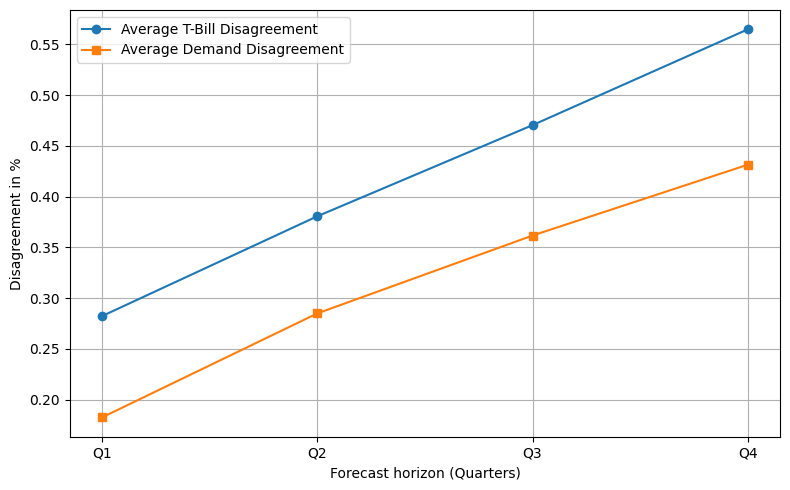
\includegraphics[width=0.5\textwidth]{figures/DemandDisagreementFigIntro.png} &
\end{tabular}
\caption{\textbf{Measuring Demand Disagreement.} This figure plots the average yield disagreement for the three-month Treasury bill and the demand disagreement across one- to four-quarter horizons. Yield disagreement is calculated as the cross-sectional standard deviation of yield forecasts, while demand disagreement is the cross-sectional standard deviation of the error terms from the regression in Equation~\eqref{regEq1}. The results show that demand disagreement accounts for a significant portion of interest rate disagreement and increases with the forecast horizon.}  \label{fig:DemandDisagreementMotivating}
\end{figure}
Figure \ref{fig:DemandDisagreementMotivating} shows that both yield and demand disagreement increase with the forecast horizon. As the horizon increases, a larger fraction of yield disagreement is captured by demand disagreement. For instance, at the one-quarter horizon, the demand disagreement is $65\%$ of the yield disagreement, but at the four-quarter horizon the demand disagreement is $76\%$. 


\section{Model}\label{sec:Model}


In this section, we present a parsimonious equilibrium overlapping generations (OLG) model with a continuum of investors who have different time preferences and beliefs. Asset price dynamics in this framework are driven entirely by demand disagreement arising from heterogeneous expectations about the future prevalence of patient and impatient investors in the economy rather than by differences in beliefs about macroeconomic fundamentals.

\subsection{Consumers, Output and Asset Markets}\label{sec:consumers}

We consider a continuous-time overlapping generations economy in the tradition of \cite{Blanchard2013} and \cite{Garleanu2008}.  Every agent lives until the stochastic time of death $\tau$ which is exponentially distributed with hazard rate, $\nu > 0$.\footnote{If $\nu=0$ agents live forever and we return to the classical infinite horizon economy.}  A continuum of agents of mass $\nu$ is born every period and therefore the total population size remains constant, that is, $\int^{t}_{-\infty}\nu e^{-\nu\left(t-s\right)}  \: ds = 1$, where $\nu e^{-\nu\left(t-s\right)}$ denotes the population density.  

We follow \cite{GarlenauKoganPanageas2012}, \cite{panageas:2020}, and \cite{GPG:2021} by letting investors born at time $t$ receive an equal share of a new ``tree'' that arrives at time $t$. The time $t$ dividend of a tree arriving at time $s \leq t$ is $Y_{s,t} = \nu e^{-\nu\left(t-s\right)}Y_t$, 
where $\nu$ denotes the depreciation rate and, therefore, the aggregate dividend, which is equal to aggregate output, at time $t$ is $\int^{t}_{-\infty}Y_{s,t} \: ds = \int^{t}_{-\infty}\nu e^{-\nu\left(t-s\right)}Y_t \: ds = Y_t.$\footnote{We set the depreciation rate to be the same as the hazard rate.} Aggregate output $Y_t$ follows a Geometric Brownian Motion, that is, $dY_{t} = \mu_{Y} Y_{t} \: dt + \sigma_{Y} Y_{t} \: dZ_{Y,t}$.
We refer to the Brownian motion $Z_{Y,t}$ as the supply shock and the constants $\mu_Y$ and $\sigma_Y$ as the expected output growth rate and output growth volatility, respectively. 

There are two types of agents with common risk-preferences but different time discount rates and beliefs. Patient type $a$ agents have the low time discount rate $\rho^a$, satisfying $\nu + \rho^a>0$ to ensure a finite wealth-consumption ratio in all states, and impatient type $b$ agents have the high time discount rate $\rho^b > \rho^a$.  The fraction of patient and impatient newborns is $\alpha_t$ and $1-\alpha_t$, respectively. Let $\alpha_t = \alpha(l_t) = 1/(1+\exp(-l_t))\in \left(0,1\right)$, where $l_t$ follows the mean reverting Ornstein-Uhlenbeck process
\begin{equation}\label{l_dynamics}
	dl_t = \kappa \left(\bar{l} - l_t\right)dt + \sigma_{l}\: dZ_{\alpha,t}, \qquad \kappa, \sigma_l >0.
\end{equation}
The Brownian motion $Z_{\alpha,t}$ is independent of the supply shock, $Z_{Y,t}$. An increase in $l_t$ increases the fraction of patient investors, and thus decreases the demand for current consumption, and thus we refer to $Z_{\alpha,t}$ as the demand shock. %Note that $\alpha_t$ and $l_t$ are positively correlated and that $\lim_{l \to \infty} \alpha(l) = 1$ and $ \lim_{l \to -\infty} \alpha_t = 0$. 

Let $P_{s,t}$ denote the value of the vintage dividend tree of time $s$ at time $t$. The instantaneous return of this stock is $dR^S_{t} = dP_{s,t}/P_{s,t} + Y_{s,t}/P_{s,t} dt$.
We drop the $s$ subscript because all stocks are perfectly correlated and thus the stock return, $R^S_{t}$, does not depend on the vintage $s$.  We will therefore refer to this ``representative'' stock as the stock market. In addition to trading stocks in positive supply, agents can trade an instantaneously risk-free asset with real short rate, $r_t$, in zero-net-supply, and a consol in zero-net-supply with the time-dependent coupon rate $e^{(\mu_Y - \sigma_Y^2 - \nu)  t}$ and price $B^{C}_t =  \int_{t}^{\infty} e^{(\mu_Y - \sigma_Y^2 - \nu) (T-t)} B^{T}_{t} \: du $, %Specifically, 
where $B^{T}_{t} $ denotes the price of a discount bond that matures at time $T$. We denote the instantaneous return of the consol bond by $dR^{C}_t$, derive its price in Corollary \ref{corollary:consol} in closed form, and show at the end of Section \ref{sec:solution}, that it is only exposed to demand shocks, $Z_{\alpha,t}$. Any other bond that is not instantaneously risk-free would also complete the market, but its price would not be given in closed form. The real short rate, the stock market diffusion coefficients, the expected stock market return, the consol diffusion coefficient, and the expected return on the consol are all determined in equilibrium.  Finally, there is an annuity contract as in \cite{Blanchard2013} and \cite{Garleanu2008} that is offered by a competitive insurance industry that pays the actuarially fair rate $\nu$ per unit of wealth. Hence, the cash flows from this annuity contract from the perspective of investors for all $t \leq \tau$ are $ d \mathcal{L}_t =  \nu W^\mathcal{L}_{t} \: dt$ with $\mathcal{L}_{\tau} = -W^{\mathcal{L}}_{\tau}$.

Agent $i \in \{a,b\}$ born at time $s$ chooses the consumption process $c^i_{s,t}$ to maximize the lifetime expected utility with respect to her belief $\mathbb{P}^i$ (determined in the next subsection)
\begin{equation} \label{EUdynamic}
	E^i_{s}\left[\int_{s}^{\tau}e^{-\rho^i \left(t-s\right)} \log\left(c^i_{s,t}\right)dt\right],
\end{equation}
subject to the dynamic budget constraint
\begin{equation} \label{wealthdynamics} 
	dW^i_{s,t} = \left(r_tW^i_{s,t} - c^i_{s,t}\right)dt + \Phi^i_{s,t}\left(dR_{t}-r_tdt\right) +\Psi^i_{s,t}\left(dR^{\alpha}_t-r_tdt\right) + d \mathcal{L}_{s,t}^i,
\end{equation}
where $W^i_{s,s} = P_{s,s}$, $W^i_{s,\tau} =W^i_{s,\tau^{-}} + \mathcal{L}_{s,\tau}^i = 0,$ and $\Phi^i_{s,t}$ and $\Psi^i_{s,t}$ denote the dollar amounts held in the stock and the consol, respectively.  

 

\subsection{Information and Beliefs}

There are two fundamental sources of heterogeneity in the model: investors differ in both their time preferences (patient vs.~impatient) and their beliefs about the prevalence of their types (optimist vs. pessimist). In principle, this would allow for four types of agents in each cohort (high/low time discount rate $\rho$, optimistic/pessimistic about $\bar{l}$). 
 To maintain tractability, we impose that each investor type believes their own preferences are more common than they actually are; a cognitive bias often referred to as the "false consensus bias" in the psychology literature (e.g. \cite{RossGreenHouse77}).\footnote{In the Internet Appendix, we show that our results are qualitatively the same if we reverse the false consensus bias to $\bar{l}^a < \bar{l} < \bar{l}^b$ and discuss the small quantitative differences it implies for unconditional asset pricing moments.} Specifically, patient investors are optimistic about the long-run mean ($\bar{l}^a \geq \bar{l}$), while impatient investors are pessimistic ($\bar{l}^b \leq  \bar{l}$). Importantly, we do not assume that either group has more accurate beliefs; rather, both patient and impatient investors are equally biased, so that $\bar{l}^a - \bar{l} = \bar{l} - \bar{l}^b$. This symmetry links time preference and belief heterogeneity, allowing us to summarize cross-sectional differences with a single endogenous state variable, the consumption share of patient investors $f_t$. 

Formally, investors observe $\alpha_t$ and thus $l_t$, but disagree about the long-run mean of $l_t$. Investors of type $i \in \{ a,b \}$  believe that $l_t$ follows 
\begin{equation}\label{l_dynamics_perceived} dl_t = \kappa\left(\bar{l}^i - l_t\right) \: dt + \sigma_{l} \: dZ^i_{\alpha,t}, \end{equation} 
where $Z^i_{\alpha,t}$ denotes the demand shock perceived by an investor with belief $\mathbb{P}^i$. The true and perceived demand shocks are linked by $Z^i_{\alpha,t} = Z_{\alpha,t} - \sigma_{\Delta}^i t$ with $\sigma_{\Delta}^i = \left(\bar{l}^i - \bar{l}\right)(\kappa/\sigma_{l})$. Investors do not learn and only disagree about the long-run mean, so $\sigma_{\Delta}^i$ is constant.\footnote{We discuss the effects of learning from experience which generates time-varying, cohort-dependent disagreement, and richer belief dynamics in Section~\ref{sec:Extensions} and the Internet Appendix.} Girsanov's theorem implies that the likelihood ratio between investor $i$'s and the data-generating belief is $\eta_t^i \equiv (d\mathbb{P}^i/d\mathbb{P})_{\mathcal{F}_t} = \exp \left(-0.5 \left( \sigma_{\Delta}^i \right)^2 t + \sigma_{\Delta}^i Z_{\alpha,t}\right)$. We capture disagreement between patient and impatient investors with the likelihood ratio:
\begin{equation}\label{eq:LR} 
    \eta_t \equiv \frac{d\mathbb{P}^b}{d\mathbb{P}^a} \mid_{\mathcal{F}_t} = \frac{\eta_t^b}{\eta_t^a} = e^{- \frac{1}{2}\sigma_{\Delta}^2 t - \sigma_{\Delta}\: Z_{\alpha,t}^a}, \qquad \text{and} \qquad 
    \sigma_{\Delta}= \sigma_{\Delta}^a - \sigma_{\Delta}^b = 2 \frac{\kappa}{\sigma_{l}} \left( \bar{l}^a - \bar{l} \right) =
     2 \frac{\kappa}{\sigma_{l}} \left(  \bar{l} - \bar{l}^b \right). 
\end{equation} 
We use the parameter $\sigma_{\Delta}\geq 0$ to quantify the degree of demand disagreement between investor types.
    
 
\subsection{Arrow-Debreu Price System} 

Before computing the equilibrium, it is convenient to summarize the price system in terms of the investor-specific state price density, $\xi^i_{t}$, which captures the investor-specific belief, but the common Arrow-Debreu price system. For example, the price of an asset with payoff $x_{t+1}$ is $p_t = \mathrm{E}^a_t \left [ \frac{ \xi^a_{t+1}}{\xi^a_t} x_{t+1} \right] = \mathrm{E}^b_t \left [ \frac{ \xi^b_{t+1}}{\xi^b_t} x_{t+1} \right].$ 
The dynamics of the state price density of investor $i \in \{ a, b \}$ are $d\xi^i_{t}  =  - r_t \xi^i_t \: dt - \theta_{Y,t} \xi^i_t  \: dZ_{Y,t} - \theta^i_{\alpha,t} \xi^i_t\: dZ^i_{\alpha,t}$,  
where $\theta_{Y,t}$ denotes the market price of supply shock risk $Z_{Y,t}$ and $\theta^i_{\alpha,t}$ denotes the market price of demand shock risk $Z^i_{\alpha,t}$ perceived by investor $i$.\footnote{Investors within a patient or impatient cohort agree on the dynamics of $\alpha_t$ and so their beliefs and, thus,  state price densities do not depend on their date of birth $s$. In Section \ref{sec:Extensions}, we discuss a model that allows investors within a cohort to learn from their experience, and thus there is a difference in beliefs between agents with the same time preferences. Full details on this model can be found in the Internet Appendix.} %In equilibrium the risk-free rate and the market prices of risk pin down the state price densities $\xi_t^a$ and $\xi_t^b$ which are determined in Theorem \ref{th:Equilibrium} below. 
Individual state price densities are linked by the likelihood ratio $\eta_t$ given in Equation (\ref{eq:LR}) and, thus, the perceived market prices of demand risk are linked through the disagreement parameter $\sigma_{\Delta}$, that is, $\xi^a_t = \eta_t \xi^b_t$ and $\theta^a_{\alpha,t}- \theta^b_{\alpha,t} = \sigma_{\Delta}$. Similarly, we present the Arrow-Debreu price system under the data generating belief by the state price density $\xi_t = \xi_t^a \eta_t^a = \xi_t^b \eta_t^b$ because the price of an asset with payoff $x_{t+1}$  can be equivalently written as $p_t = \mathrm{E}_t \left [ \frac{ \xi_{t+1}}{\xi_t} x_{t+1} \right]$ with $d\xi_{t} =  -r_t\xi_t - \theta_{Y,t}\xi_t dZ_{Y,t}- \theta_{\alpha,t}\xi_t dZ_{\alpha,t}$ and $\theta_{\alpha,t}  = \theta^i_{\alpha,t} - \sigma_{\Delta}^{i}$.

\section{Equilibrium}\label{sec:solution}


In this section, we solve for the equilibrium that is defined in a standard way. That is, given preferences, endowments, and beliefs, an equilibrium is a collection of allocations and a price system such that all agents maximize their expected lifetime utility and all markets clear. As soon as agents are born, they face a dynamically complete security market because the four securities described in the previous section allow agents to share supply shock, demand shock, and mortality risk. Hence, instead of solving the consumption-portfolio choice problem given in equations (\ref{EUdynamic}) and (\ref{wealthdynamics}) for each agent, we can solve for the equilibrium by using the martingale methods developed in \cite{KaratzasLehoczkyShreve1987} and \cite{Cox1989}. The static optimization problem is 
\begin{equation}\label{eq:StaticP}
     \underset{\{ c^i_{s,t}: \: s \leq t  \}}{\max} \quad E^i_{s}\left[\int_{s}^{\infty}e^{-\left(\rho^i + \nu \right) \left(t-s\right)} \log\left(c^i_{s,t}\right)dt\right]  \qquad
\text{s.t.} \qquad 
E^i_{s}\left[\int_{s}^{\infty}e^{-\nu \left(t-s\right)} \frac{\xi^i_{t}}{\xi^i_{s}}   \left(c^i_{s,t}-Y_{t} \right) \: dt\right] = 0.
\end{equation}
The time of death $\tau$ is exponentially distributed, and thus we solve an infinite-horizon problem where the finite life effectively increases the time discount rate from $\rho^i$ to $\rho^i + \nu$. Solving the FOC of the static optimization problem given in Equation (\ref{eq:StaticP}) for individual consumption leads to

\begin{equation}\label{optimalconsumption}
 c^i_{s,t} =c^i_{s,s} e^{-\rho^i \left(t-s\right)} \frac{\xi^i_{s}}{\xi^i_{t}}, \quad \forall \: s \leq t \leq \tau^i \qquad \text{with} \qquad c^i_{s,s} = \frac{1}{\kappa^i_s}, \qquad  i \in \{ a,b\}.
\end{equation}
The individual consumption growth rate is inversely related to the investor's time discount rate and to the state price density. Moreover, the initial consumption share is inversely related to the Lagrange multiplier of the static budget constraint, $\kappa^i_s$, and needs to be solved in equilibrium because agents cannot hedge against endowment fluctuations prior to birth and thus initial consumption varies with the value of the endowment stream. 
 
The total wealth at time $t$ of a consumer of type $i$ born at time $s$, $W^i_{s,t}$ is equal to the value of the consumption stream at time t. Specifically, $W^i_{s,t} = E^i_{t}\left[\int_{t}^{\infty}  e^{-\nu \left(u-t\right)}  \frac{\xi^i_{u}}{\xi^i_{t}}  c^i_{s,u} \: du\right] = \frac{1}{\rho^i+\nu} c^i_{s,t}$. Hence, the individual consumption-wealth ratio is constant and equal to the effective subjective time discount rate, that is, $c^i_{s,t}/W^i_{s,t} = (\rho^i+\nu)$.
Initial wealth is equal to the total wealth in the economy, i.e., $W^i_{t,t}  = P_{t,t} = W_t$.\footnote{Define $\hat{Y}_{s,t}$ as the total endowment of all agents born up until time $s \leq t$. The total wealth at time $s$ is the value of this endowment stream. We have $\hat{Y}_{s,t} = e^{-\nu\left(t-s\right)}Y_t$, which is equivalent to the endowment of an agent born at time $s$. Hence, their valuations are the same as well.} The initial individual consumption share of agent i at time t is 
\begin{equation} \label{eq:beta}
	\beta^i_t \equiv  \frac{c^i_{t,t}}{Y_t} =\left(\rho^i + \nu\right)\phi_t, \qquad \forall \: i \in \lbrace a, b \rbrace, 
\end{equation} 
where $\phi_t = \frac{W_t}{Y_t}$ is the aggregate wealth-consumption ratio. Hence, consumers born in times of high valuations have a higher welfare weight and consume more than consumers born in times of low valuations. 

To derive the equilibrium, we proceed as follows. First, we solve for the stochastic discount factor as a function of the consumption share, $f_t$, the fraction of patient agents, $\alpha_t$ and the initial individual consumption shares $\beta^a_{t}$ and $\beta^b_{t}$. Finally, we show that the wealth-consumption ratio is a consumption share weighted average of the wealth-consumption ratios in the two homogeneous agent economies, allowing us to determine the initial consumption shares $\beta^a_{t}$ and $\beta^b_{t}$.  To solve for the  equilibrium stochastic discount factor, we insert the optimal consumption from Equation (\ref{optimalconsumption}) into the aggregate resource constraint, $\int_{-\infty}^{t} \nu e^{-\nu (t-s )} (\alpha_s c^a_{s,t}+(1-\alpha_s) c^b_{s,t}) ds =  Y_t$. The result is presented in the next proposition.
\begin{prop}[Stochastic discount factor]\label{SDF}
The equilibrium stochastic discount factor is $\xi_t = \frac{X_t}{Y_t}$ with $X_t =\int_{-\infty}^{t} \nu e^{-\nu \left(t-s\right)} \left(\alpha_s \beta^a_s e^{-\rho^a \left(t-s\right)}\frac{\eta^a_t}{\eta^a_s} +\left(1-\alpha_s\right)\beta^b_s e^{-\rho^b \left(t-s\right)} \frac{\eta^b_t}{\eta^b_s}\right)X_s \: ds$.
\end{prop}
The stochastic discount factor in Proposition \ref{SDF} is inversely related to aggregate output as in a standard infinitely lived representative agent economy with log utility and depends on the process $X_t$ which captures variations in state prices due to differences in time discount rates and beliefs. To study the effects of this heterogeneity on asset prices, we define the consumption share of patient and impatient investors. Specifically, $f_t  = \int_{-\infty}^t \nu  e^{-\nu(t-s)}  \alpha_s (c_{s,t}^a/Y_t) \: ds$ and $1-f_t  = \int_{-\infty}^t \nu  e^{-\nu(t-s)}  (1-\alpha_s) (c_{s,t}^b/ Y_t) \: ds$, respectively.  
The endogenous consumption share $f_t$ and the exogenous process $\alpha_t$ are the two state variables that describe all the variation in asset prices.  The consumption share is presented in the next proposition. 
\begin{prop}[Consumption shares]\label{prop:f}
The consumption shares are $f_t = X^a_t/X_t$ and $1-f_t = X^b_t/X_t$ with $X^a_t = \int_{-\infty}^{t} \nu e^{-\left(\rho^a + \nu\right)\left(t-s\right)}\alpha_s \beta^a_s (\eta^a_t/\eta^a_s)X_s ds$ and $X^b_t = \int_{-\infty}^{t} \nu e^{-\left(\rho^b + \nu\right)\left(t-s\right)}\left(1-\alpha_s\right) \beta^b_s (\eta^b_t/\eta^b_s)X_s ds.$
\end{prop}
Applying Ito's lemma to the stochastic discount factor $\xi_t = \frac{X_t}{Y_t}$ and matching the drift and the diffusion coefficients leads to the equilibrium real short rate and market prices of risk presented in Proposition \ref{prop_rtandtheta}. 
 \begin{prop}[Risk-free rate and market prices of risk]\label{prop_rtandtheta}
In equilibrium, the real short rate is 
\begin{equation}\label{rt}
    r_t =  \mathcal{E}_{f}\left [ \rho \right]  + \mu_Y - \sigma_Y^2 + \nu\left(1 - \alpha_t \beta^a_t - \left(1-\alpha_t\right)\beta^b_t\right),
\end{equation}
with market time discount rate $\mathcal{E}_{f}\left [ \rho \right] = f_t \rho^a + \left(1-f_t\right)\rho^b$. The market price of output risk is $\theta_{Y,t} = \sigma_Y$ and the market price of demand shock risk is
\begin{equation}\label{theta_alphat}
	\theta_{\alpha,t}  = -\mathcal{E}_{f}\left [ \sigma_{\Delta}  \right]  = \frac{\kappa}{\sigma_l} ( 
	\bar{l} - \mathcal{E}_{f}\left[\bar{l} \right] ) 
	=  \sigma_{\Delta}\left(\frac{1}{2} - f_t \right).
\end{equation}
with market views $\mathcal{E}_{f}\left[\bar{l} \right]= \bar{l}^a f_t + \bar{l}^b  ( 1- f_t  )$ and $\mathcal{E}_{f} \left [ \sigma_{\Delta} \right] = f_t \sigma_{\Delta}^a  + \left(1-f_t\right)\sigma_{\Delta}^b$.\footnote{For a detailed discussion of the market view, see \cite{HLI2025}.}
\end{prop}
There are four economic effects that determine the risk-free interest rate: (i) a time-discounting effect, (ii) an intertemporal substitution effect, (iii) a precautionary savings effect, and (iv) an effect of the OLG structure. The market time discount rate, $\mathcal{E}_{f}\left [ \rho \right]$ is the consumption share weighted average of the patient ($\rho^a$) and impatient ($\rho^b$) investors' time discount rates.  The risk-free rate is inversely related to the consumption share of patient investors ($f_t$) because when $f_t$ is high, the risk-free rate $r_t$ is low to discourage excessive savings by patient investors, ensuring equilibrium of the bond market. The intertemporal smoothing and precautionary saving effects are captured by the term $\mu_Y - \sigma_Y^2$, and are the same as in a standard infinitely lived representative agent economy with log utility. The effect of the OLG structure is captured by the term $ \nu\left(1 - \alpha_t \beta^a_t - \left(1-\alpha_t\right)\beta^b_t\right)$. If there is no time-preference heterogeneity, then this term is zero. This is no longer the case with preference heterogeneity as the expected consumption growth of agents currently alive no longer coincides with expected output growth. Hence, a displacement effect must be taken into account because the short-term interest rate reflects only expected consumption growth from agents currently alive. Specifically, if agents who are currently alive are expected to consume less on average than agents that are born next period, then the effective consumption growth is lower, and, therefore, the interest rate is also lower. Disagreement about the process $\alpha_t$ does not directly affect the real short rate. However, it significantly influences the distribution of the risk-free rate through its impact on the consumption share ($f_t$) and the relative consumption of newborns ($\beta^i_t$) as discussed in more detail in Section \ref{sec:analysis}.\footnote{To isolate the effects of demand disagreement on asset prices, we assume that $Y_t$ and $\alpha_t$ are independent; if they were correlated, the real short rate $r_t$ would depend directly on disagreement.}

The market price of output shocks (\(\theta_{Y,t} = \sigma_Y\)) is the same as in a standard log-utility economy. However, the price of demand shocks (\(\theta_{\alpha,t}\)) depends on the market view of \(\bar{l}\), represented by the consumption-share-weighted average belief \(\mathcal{E}_{f}\left[\bar{l}\right]\) rather than the statistical view \(\bar{l}\). Demand shocks are not priced only when the market view aligns with the statistical view, which occurs if patient and impatient investors have equal consumption shares (\(f_t = 0.5\)). When impatient investors consume a larger share (\(f_t < 0.5\)), their beliefs have more impact, resulting in a positive market price of demand shock risk (\(\theta_{\alpha,t} > 0\)). In contrast, when patient investors have a larger consumption share, the market price of demand risk turns negative. The intuition is straightforward: impatient investors, who overestimate future demand for consumption and, respectively, underestimate future demand for savings (lower \(\alpha_t\)), short the consol, while patient investors, who underestimate it, go long. When impatient investors consume more, the price of the consol falls to clear the market, making it appear underpriced to an econometrician who is endowed with the statistical view, thus implying a positive covariance with the pricing kernel and a positive market price of demand risk. In contrast, if patient investors have a larger consumption share, they increase the price of the consol, making it appear overpriced to the econometrician, who then perceives a negative risk premium.\footnote{This intuition is similar to \cite{MillerEdward1977} where short-sale constraints prevent pessimists from trading on their views, so the market view places greater weight on optimists’ beliefs and the stock appears overpriced to an outside observer endowed with the statistical view.}

To fully characterize the equilibrium stochastic discount factor, we need to derive the wealth-consumption ratio, $\phi_t$, as $\beta^i_t = \left(\rho^i + \nu\right)\phi_t$. The following proposition shows that $\phi_t$ is a consumption share weighted average of the wealth-consumption ratios in homogeneous agent economies with only type a or b investors. %The terms wealth-consumption ratio and price-dividend ratio are used interchangeably to refer to $\phi_t$.
\begin{prop}[Wealth-consumption ratio]\label{prop_PD}
Let $\phi^{a} \equiv \frac{1}{\rho^a+\nu}$ and $\phi^{b} \equiv \frac{1}{\rho^b+\nu}$ with $\phi^{a} > \phi^{b}$. Then the equilibrium wealth-consumption ratio is $\phi_t = \phi^{a}  f_t  + \phi^{b}  (1-f_t)  = \phi^{b} + \left( \phi^{a}-\phi^{b}\right)f_t.$
\end{prop}
The risk-free rate $r_t$, the market price of demand shocks $\theta_{\alpha,t}$, and the wealth-consumption ratio are all affine functions of the economy's sole endogenous state variable: the consumption share $f_t$. The following corollary establishes the sign of their exposure to changes in $f_t$. This result will be particularly useful in Section \ref{sec:analysis}, where we analyze the unconditional distributions of the risk-free rate, the market price of demand shock risk, and the wealth-consumption ratio, as these inherit properties from the unconditional distribution of the consumption share.

\begin{corollary}\label{corollary:affine}
The risk-free rate is strictly decreasing in the consumption share, that is, $\frac{\partial r(f)}{\partial f} = \left(\rho^a-\rho^b\right) - \nu \mathcal{E}_{\alpha} \left [ \rho \right] \left(\phi^a-\phi^b\right)<0$. The market price of demand shocks is strictly decreasing in the consumption share, that is, $\frac{\partial \theta_{\alpha}(f)}{\partial f}= - \sigma_{\Delta}$. The wealth-consumption ratio is strictly increasing in the consumption share, that is, $\frac{\partial \phi(f)}{\partial f}= \phi^{a}-\phi^{b} $.
\end{corollary}

We conclude this section with Corollary \ref{corollary:consol} which shows that the price of the consol bond coincides with the wealth-consumption ratio. Moreover, it decomposes the exposure of the stock return into cash flow and consol exposure since the wealth-consumption ratio and the price-dividend ratio coincide.
\begin{corollary}[Consol price and stock return]\label{corollary:consol}
The price of the consol is the same as the wealth-consumption ratio, that is, $B^{C}_{t} = \phi_t$. The stock return is exposed to cash flow growth, and the consol return
\begin{equation}\label{eq:stockdecompbond}
    d \log \: P_{s,t} = \underbrace{d \log \: Y_{s,t}}_{\text{\tiny cash flow exposure}} + \underbrace{d \log B^{C}_{t} }_{\text{\tiny exposure to consol}}.  
\end{equation}

\end{corollary}

 
The first term shows that the price of the stock is exposed to the supply shock $Z_{Y,t}$ through the cash flows, and the second term shows that the price of the stock is exposed to the demand shock $Z_{\alpha,t}$ through the consol. Hence, the instantaneous risk-free asset, the stock, and the consol are sufficient to complete the asset market driven by the two Brownian shocks $Z_{Y,t}$ and $Z_{\alpha,t}$. 


\section{Analysis} \label{sec:analysis}

In this section, we analyze the equilibrium derived in the previous section and show how the model is consistent with both the correlation puzzle and the disagreement correlation puzzle while at the same time reproducing many stylized asset pricing facts.

\subsection{Parameters}

The model has a total of nine parameters $\left(\mu_Y, \sigma_Y, \nu, \rho^a, \rho^b, \kappa, \bar{l}, \sigma_l, \sigma_{\Delta}\right)$. We set expected output growth to $\mu_Y=2\%$ and output growth volatility to $\sigma_Y = 3.3\%$, which is similar to the estimates in \cite{campbell-cochrane:99} that are based on a long data sample. The birth and death intensity is set to, $\nu = 2\%$  which implies an expected life of 50 years from the start of trading, as in  \cite{Garleanu2008}. We assign a time preference parameter of $\rho^a = -0.015$ to the patient type $a$ agent, ensuring a positive effective time discount rate of $\rho^a + \nu = 0.005$. The impatient type $b$ agent has a time preference parameter of $\rho^b = 0.025$. In the literature, time preferences parameters vary substantially. For example, the time preference parameters in \cite{bansal-yaron:04}, \cite{chan-kogan:02},  and \cite{campbell-cochrane:99} are $2.4\%$, $5.2\%$, and $11.6\%$, respectively. For comparison, the $5\%$ and $95\%$ percentiles of the annualized time discount factor in \cite{ALBUQUERQUE2016} are $-6.4\%$ and $11.2\%$ with a mean of $2.4\%$. 
In order to capture a slow moving change in the composition of types with a long run average for $\alpha_t$ of $50\%$, we set the parameters of the process $l_t$ as follows: long run mean $\bar{l}=0$, local volatility $\sigma_l=0.1$, and speed of mean reversion $\kappa=0.01$.\footnote{The long-run average of $\alpha$ is not precisely 0.5 when $\bar{l}=0$ due to a Jensen's correction term, but its impact is minimal.} To examine the impact of varying levels of demand disagreement on asset prices, we explore different parameter values for $\sigma_{\Delta}$ ranging from zero ($\sigma_{\Delta}= 0$), indicating no disagreement, to $\sigma_{\Delta}= 0.8$, our baseline parameter choice. Demand disagreement is not directly observable, so we estimate it using survey data as described earlier. Figure \ref{fig:DemandDisagreementYieldModelAndData} shows the average implied demand disagreement from both the data and the model across forecast horizons of one to four quarters. The results show that the disagreement is greater for longer forecast horizons, both in the model and in the data. Furthermore, the model generates modest disagreement levels compared to the data, except when $\sigma_{\Delta}= 0.8$. At the one-year horizon, the model aligns closely with the data when $\sigma_{\Delta}= 0.8$, designating it as the base case.\footnote{The Internet Appendix includes additional calibrations, considering different $\rho^a$ and $\rho^b$ values alongside various $\sigma_{\Delta}$ levels. Although such calibrations yield results similar to the base case, they show lower equity premium, bond risk premia, and volatilities.} Finally, in the base case with $\sigma_{\Delta}= 0.8$, the mean, standard deviation and autocorrelation of the pricing relevant time discount factor, $\mathcal{E}_{f}\left [ \rho \right]$, is $1.3\%$, $1.2\%$ and $0.92$ at an annual horizon.\footnote{For comparison, in the representative agent model of \cite{ALBUQUERQUE2016} with stochastic time preferences, the time preference process has a mean, standard deviation and autocorrelation at the annual horizon of $2.4\%$, $1.5\%$ and $0.9$.}

\begin{figure}[htbp]
\centering
\vspace{0.1in}
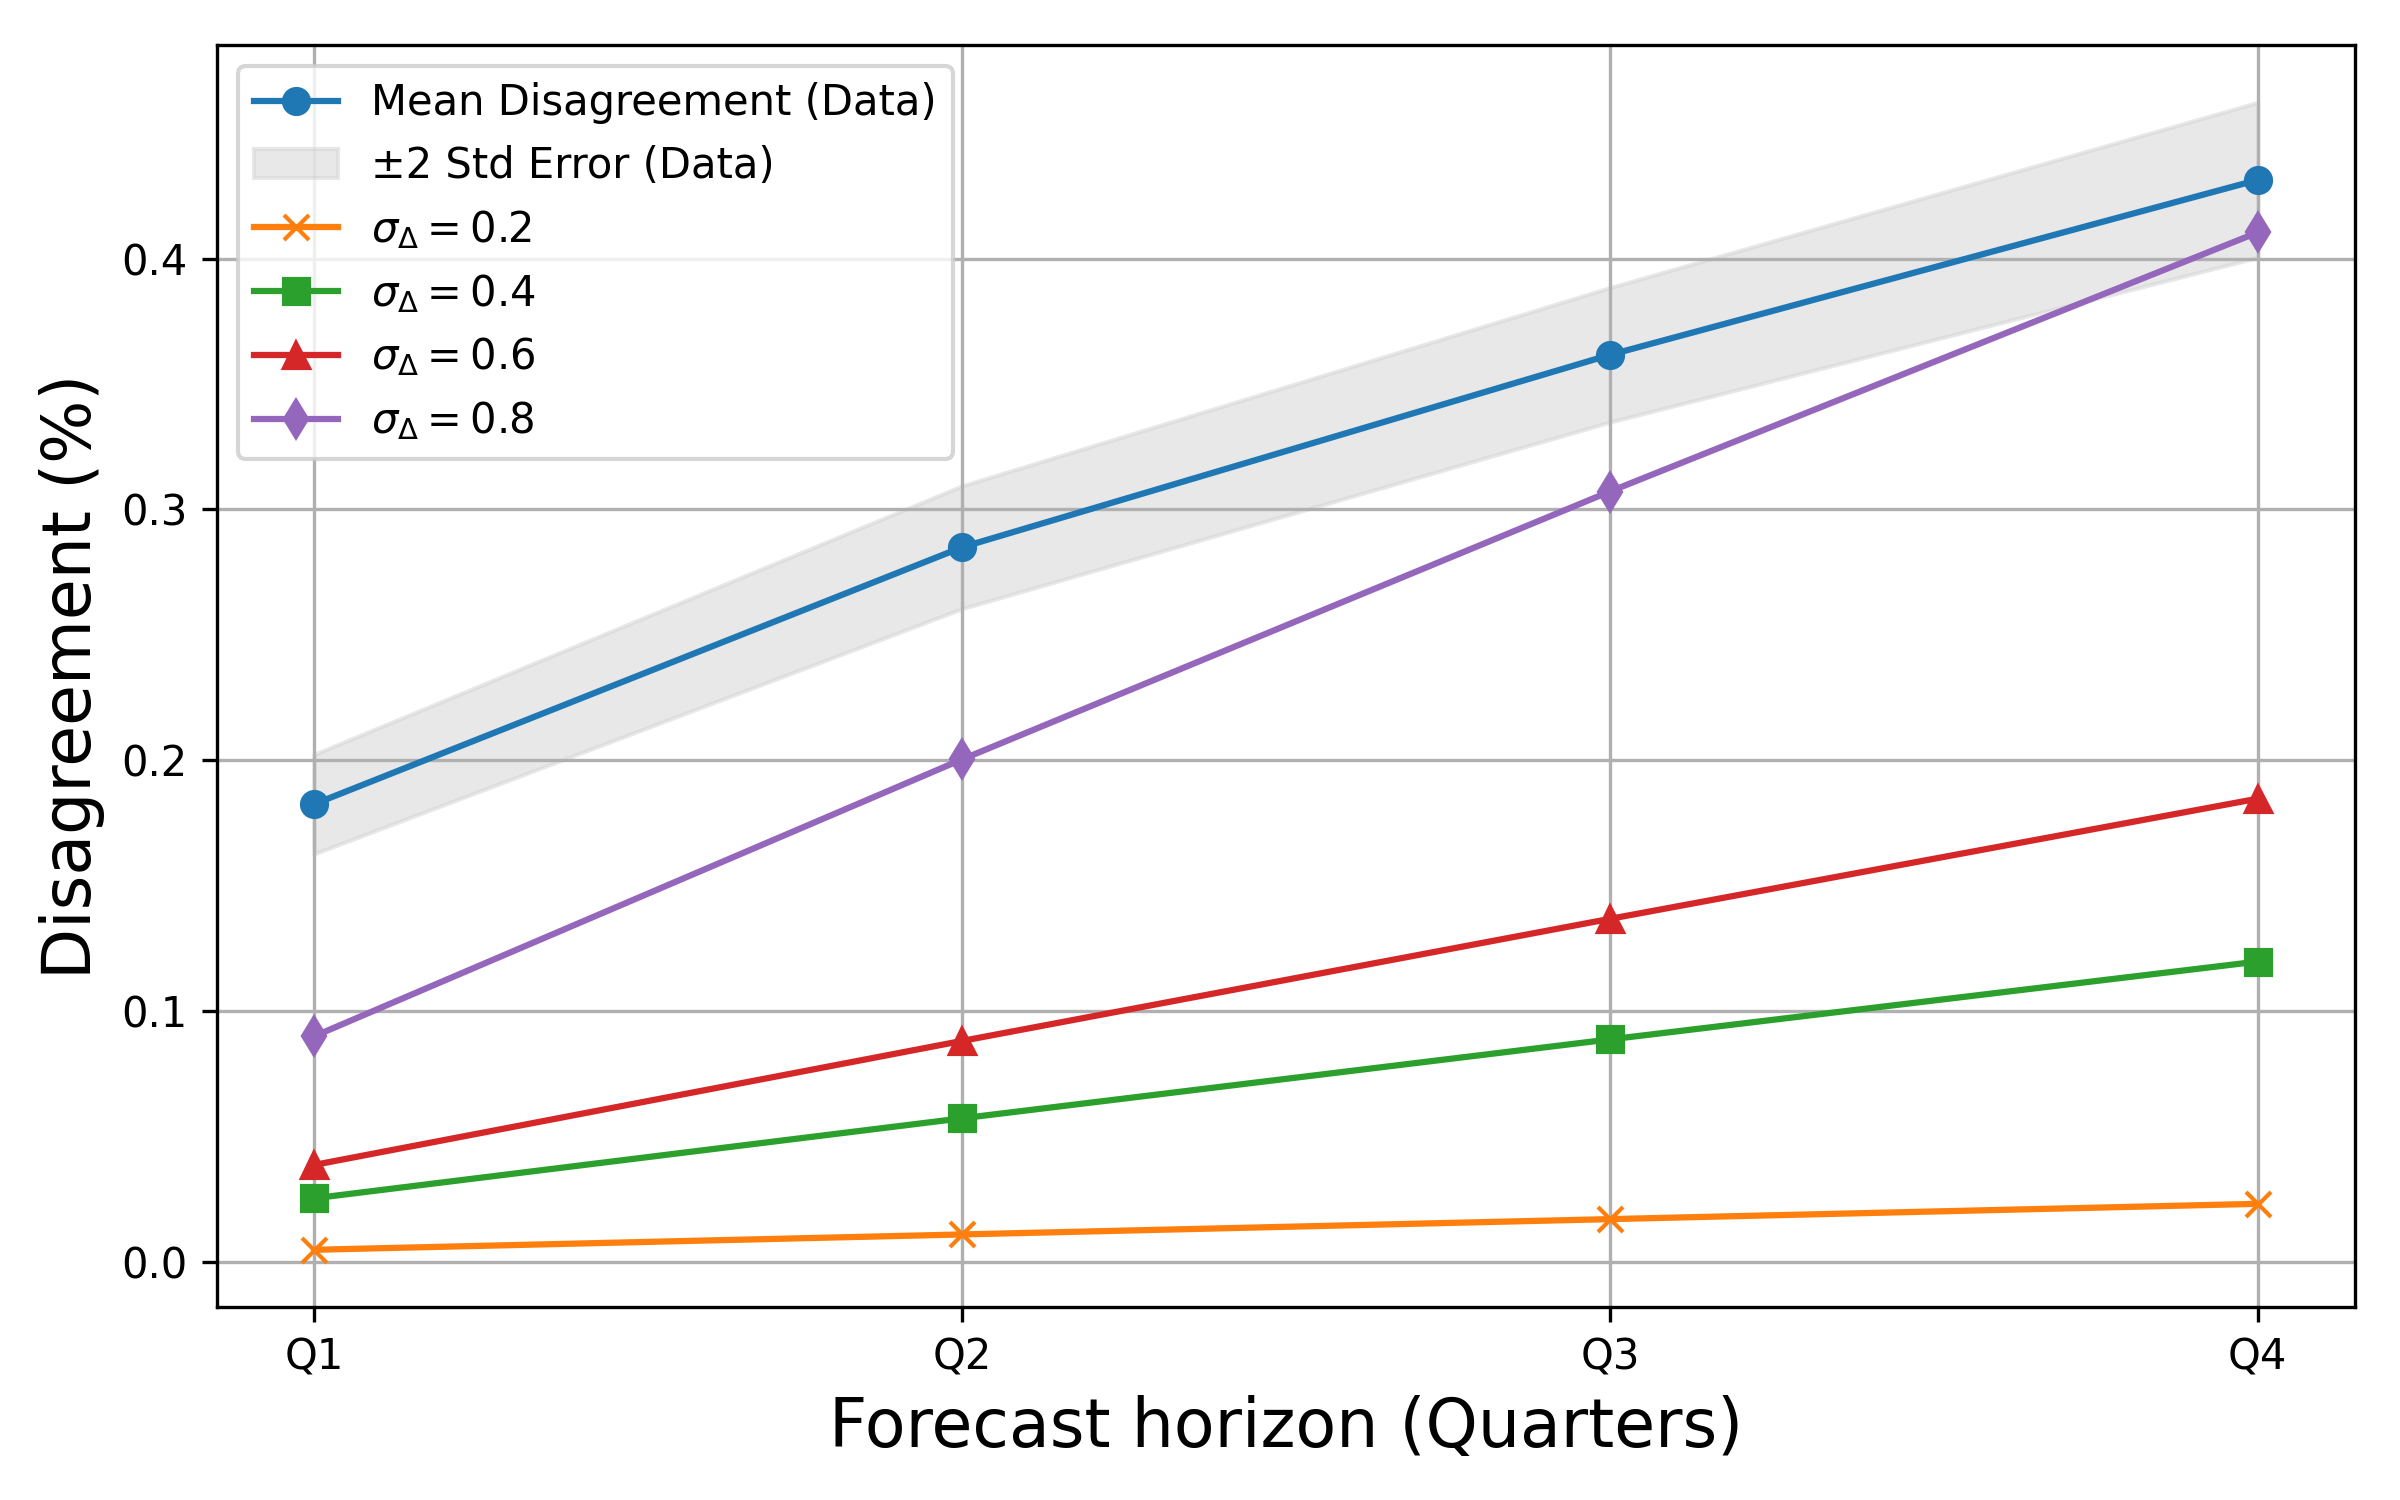
\includegraphics[width=.5\textwidth]{figuresJFE/MeanDisagreementDataAndModel.png} 
\caption{\textbf{Yield Disagreement due to Demand Disagreement.} \footnotesize{This figure compares yield disagreement due to demand disagreement in both the model and data across forecast horizons of one to four quarters. Yield disagreement is measured as the cross-sectional standard deviation of residuals from individual yield forecasts based on macroeconomic fundamentals (Section \ref{sec:empirics}). In the model, yield disagreement is derived from the cross-sectional standard deviation of real short rate forecasts by patient and impatient agents at four demand disagreement levels ($\sigma_{\Delta}= 0.2, 0.4, 0.6, 0.8$), all below empirical observations. Consequently, $\sigma_{\Delta}=0.8$ is selected as the baseline level for demand disagreement in subsequent analysis.}} \label{fig:DemandDisagreementYieldModelAndData} 
\end{figure}

 

 
\subsection{Asset Pricing Moments}\label{sec:APmoments}  

Before detailing the economic mechanism of our demand disagreement model, we first present key unconditional asset pricing moments as a function of demand disagreement $\sigma_{\Delta}$. We denote by $\tilde{\alpha}  = 1/(1+\exp(-\tilde{l}))$ the long-run fraction of newborn patient agents and by $\tilde{f}$ their consumption share, both drawn from their unconditional distributions. For each level of demand disagreement, $\sigma_{\Delta}$, we simulate $500,000$ years of monthly data for $l_t$, which follows the dynamics given in Equation~(\ref{l_dynamics}), and for $f_t$, which follows the dynamics specified in Proposition~\ref{prop:df} below. Figure \ref{fig:UnconditionalAP} shows the unconditional mean and volatility of asset price moments based on $\tilde{\alpha}$ and $\tilde{f}$, while Figure \ref{fig:ConsumptionShare} presents a histogram of the consumption share $\tilde{f}$.  

\begin{figure}[htbp]
\centering
\vspace{0.1in}
\begin{tabular}{cc}
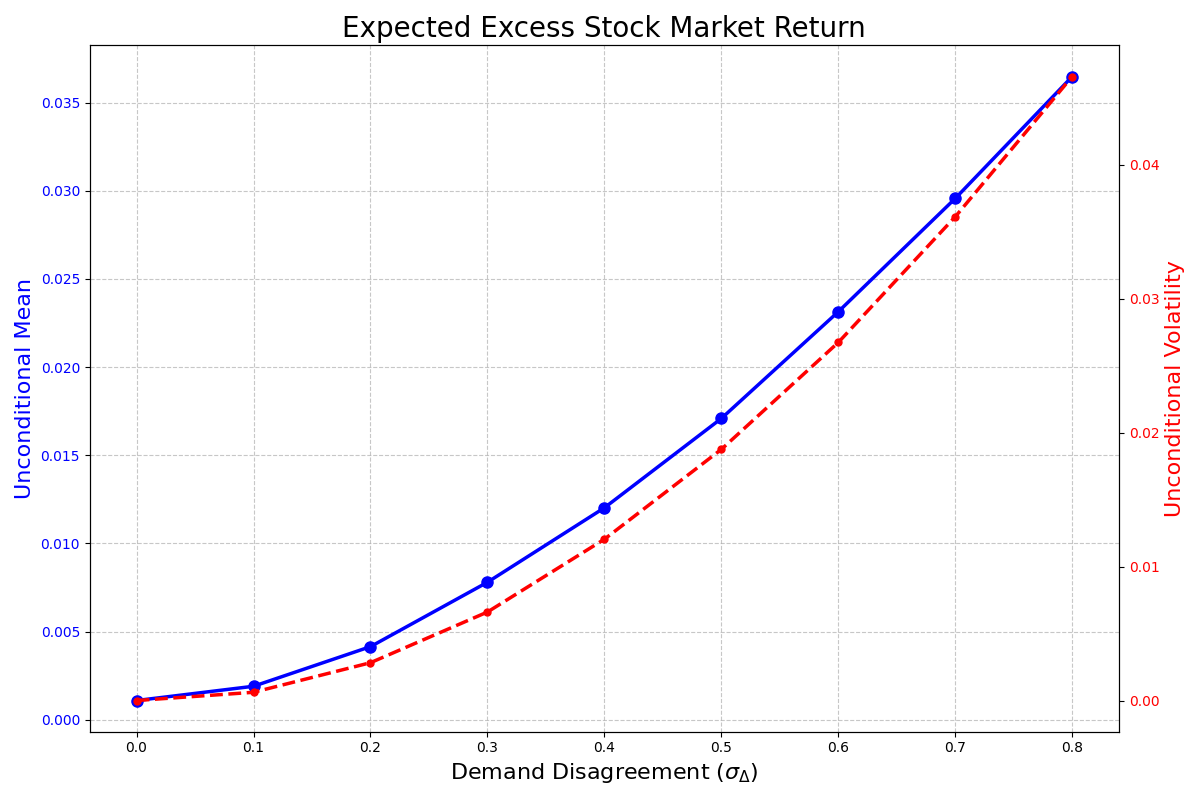
\includegraphics[width=.4\textwidth]{figuresJFE/APUnconditionalExcessReturnsJFE.png} &
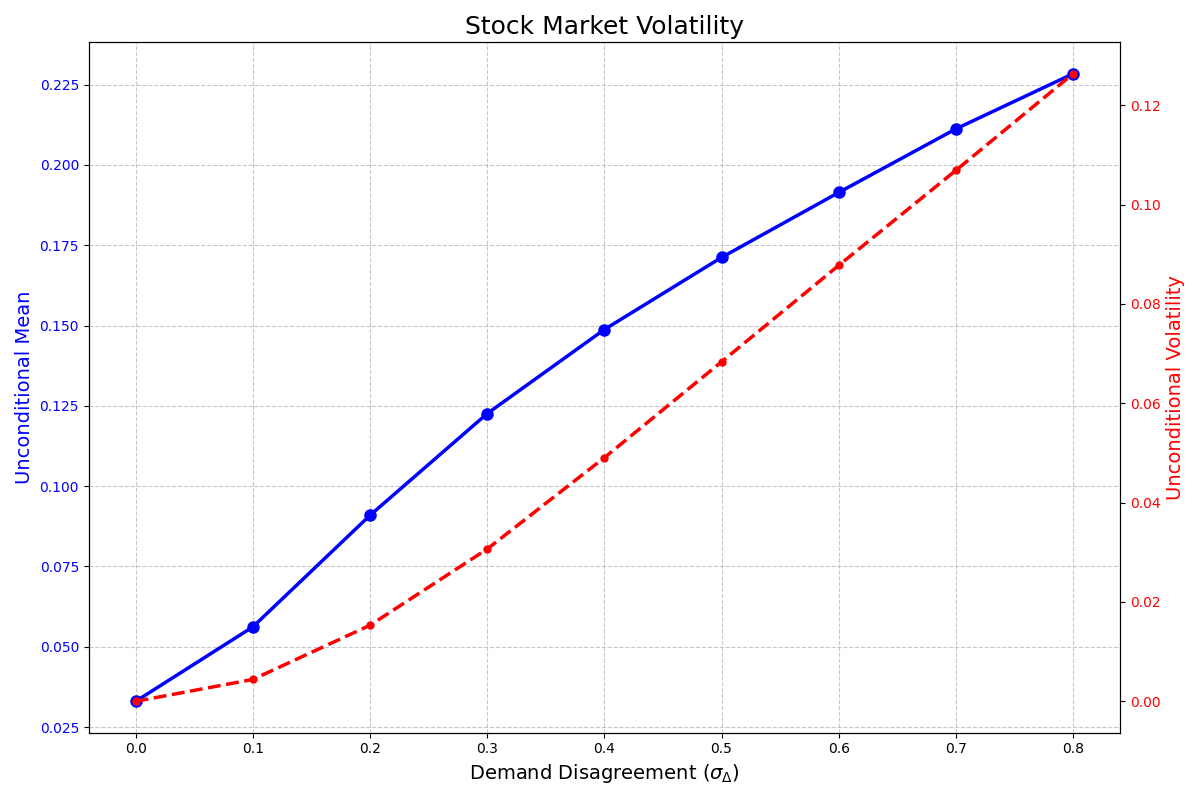
\includegraphics[width=.4\textwidth]{figuresJFE/APUnconditionalStockMarketVolatilityJFE.png} \\
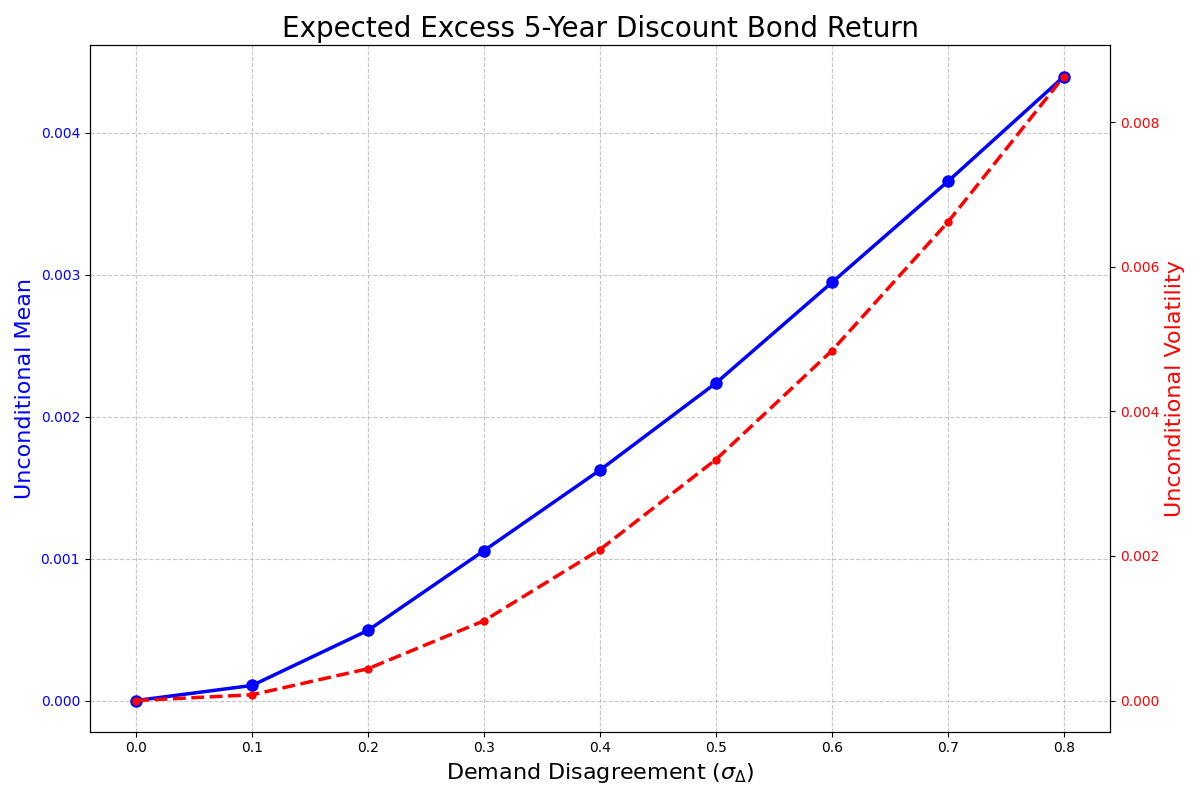
\includegraphics[width=.4\textwidth]{figuresJFE/ExRBond5yearJFE.png} &
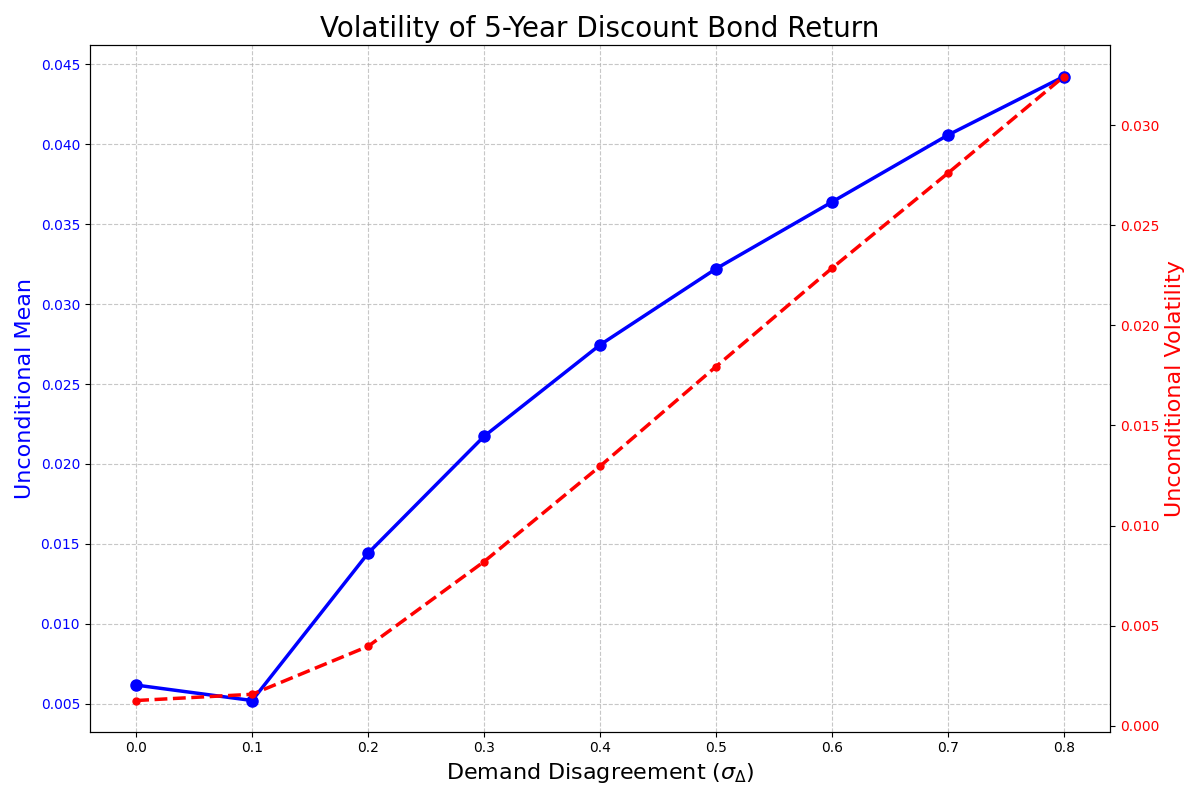
\includegraphics[width=.4\textwidth]{figuresJFE/BondVola5yearJFE.png} \\
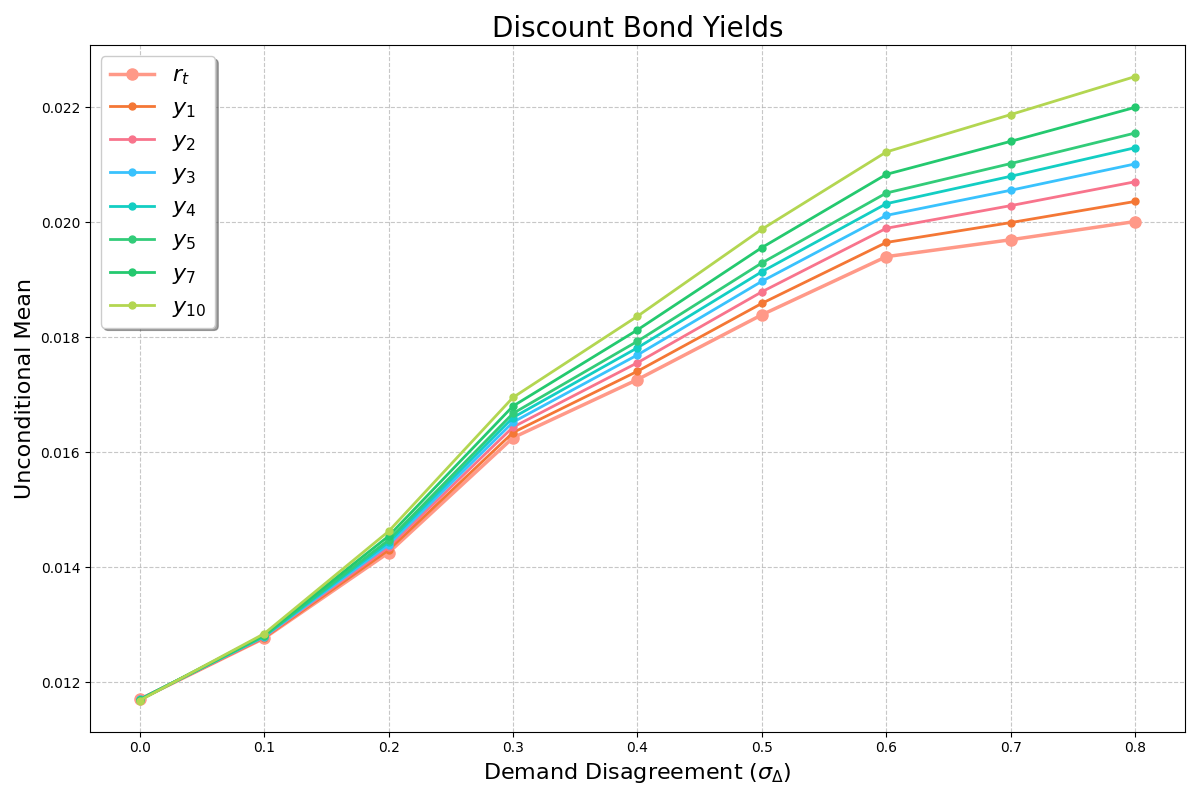
\includegraphics[width=.4\textwidth]{figuresJFE/UnconditionalYieldsJFE.png} &
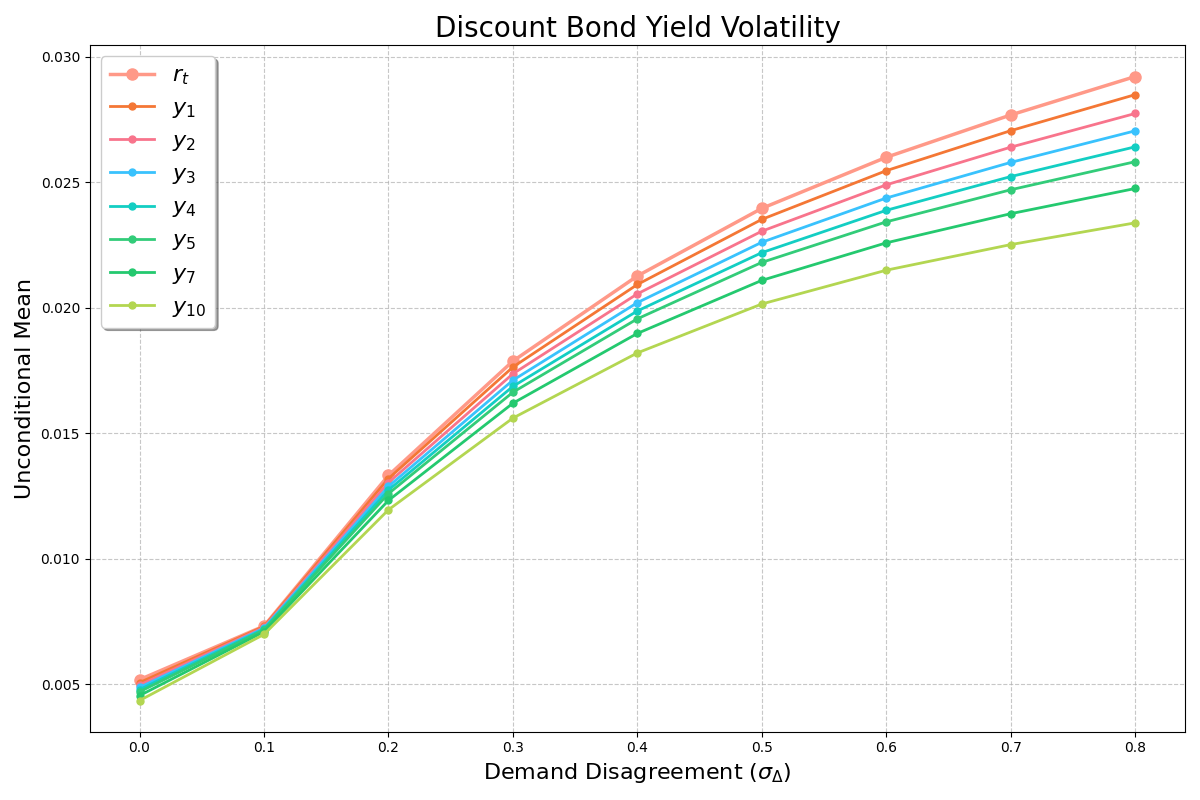
\includegraphics[width=.4\textwidth]{figuresJFE/UnconditionalYieldVolatilitiesJFE.png} \\ 
\end{tabular}
\caption{\textbf{Unconditional Asset Pricing Moments.} \footnotesize{This figure presents six key asset pricing moments: expected excess stock market return (top-left), stock market volatility (top-right), excess return on five-year bonds (middle-left), five-year bond return volatility (middle-right), the yield curve (bottom-left), and yield volatility (bottom-right). These moments are derived from simulated unconditional distributions of $\tilde{\alpha}$ and $\tilde{f}$ across various demand disagreement levels ($\sigma_{\Delta}$), based on $500,000$ years of monthly model simulations. Demand disagreement increases expected stock and bond returns, yields, the slope of the term structure, and yield volatilities.}}  \label{fig:UnconditionalAP} 
\end{figure}
Figure \ref{fig:UnconditionalAP} illustrates how increasing demand disagreement \( \sigma_{\Delta}\) affects key asset pricing moments. As \( \sigma_{\Delta}\) rises, the stock market's risk premium and volatility both increase (top-left and top-right panels), as do the risk premium and volatility of a 5-year discount bond (middle-left and middle-right panels). Similarly, yields across maturities of one to five years and their volatilities rise with disagreement, and rising $\sigma_{\Delta}$ also leads to a steeper yield curve (bottom-left and bottom-right panels).

For the baseline calibration with \( \sigma_{\Delta}= 0.8 \), the stock market risk premium is \( 3.6\% \), and the stock market volatility is \( 22.8\% \). While the risk premium is lower than the historical equity premium observed in postwar U.S. data, it is significantly higher than the no-disagreement value of \( 0.11\% \). Achieving an increasing risk premium with higher disagreement is typically challenging in models with disagreement, whereas increasing volatility is more common.\footnote{Disagreement does not always lead to excess volatility. For example, in a model with disagreement about dividends and CRRA utility with \(\gamma > 1\), cash flow volatility can exceed stock volatility (see \cite{}).}  However, our model  exhibits a risk premium that rises with increasing disagreement. The intuition behind this result is that when the market price of demand shock risk is high, the stock and bond loadings on demand shocks are also high; conversely, when the price is low or negative, their exposures are low.  We discuss this novel mechanism in detail in Section \ref{sec:analysis}.\ref{sec:StockBondDynamics}.

 The middle panels show that both the risk premium and return volatility of the 5-year bond increase with disagreement. This similar behavior in the bond and stock markets follows from Equation \eqref{eq:stockdecompbond}. Specifically, stock returns are exposed to fundamental shocks through cash flow risk and to demand shocks through their exposure to the price risk of the consol bond. Since disagreement is independent of fundamental shocks, all effects from disagreement manifest through the consol bond.

The bottom left panel shows that as disagreement increases, the slope of the yield curve becomes steeper. Our model with demand disagreement thus generates an unconditionally upward-sloping yield curve. This happens because a higher disagreement decreases the demand for long-term bonds, increasing their yields relative to short-term bonds, and steepening the yield curve. We will provide more intuition for the increase of risk premia and the steeping of the yield curve with rising demand disagreement in Section \ref{sec:analysis}.\ref{sec:StockBondDynamics}.

In addition, as disagreement increases, the volatility of risk premia in both the stock and bond markets increases. While this may not be surprising, it is significant because these premia are not constant in the data. More importantly, as we show in Section \ref{sec:analysis}.\ref{sec:backout}, demand disagreement predicts future bond returns and variations in bond return volatility in both our model and the data.\footnote{Earlier versions of this paper focused on stock markets, showing that demand disagreement predicts higher future stock returns when the price-dividend ratio is low and explains Black's leverage effect. These results are now reported in the Internet Appendix, as our main focus has shifted to bond markets.}



\subsection{Economic Mechanism -- The Consumption Share}

In this section, we analyze the economic mechanism underlying the demand disagreement model, focusing on its two state variables: the exogenous fraction of the newborn patient agents, $\alpha_t$ and the endogenous consumption share of the patient agents, $f_t$. The following proposition presents the dynamics of the endogenous state variable, $f_t$, to further clarify its properties. 
\begin{prop}[Consumption Share Dynamics]\label{prop:df}
The dynamics of the consumption share of patient agents, $f_t$, in equilibrium are $df_t = \mu_{f,t} \: dt + \sigma_{f,t} \: dZ_{\alpha,t}$ with
\begin{equation}
  \begin{split}
	\label{eq:muf}
	\mu_{f,t} &= \nu\left(\alpha_t \beta^a_t \left(1-f_t\right) - \left(1-\alpha_t\right)\beta^b_t f_t\right) + \left(\rho^b-\rho^a\right)f_t\left(1-f_t\right) \\ 
	&+ \sigma_{\Delta}^2 \left( \frac{1}{2} - f_t \right) f_t\left(1-f_t\right) 
	\qquad \text{and} \qquad \sigma_{f,t} = f_t (1-f_t) \sigma_{\Delta}. 
  \end{split}
\end{equation}
\end{prop}

Output shocks do not affect the consumption share because investors have the same risk preferences and agree on the output shock, and thus have the same exposure to output shocks.  The left graph of Figure \ref{fig:ConsumptionShare} shows the volatility of the consumption share, $\sigma_{f,t}$, as a function of the consumption share, $f_t$, for different disagreement $\sigma_{\Delta}$.  There are no shocks to the consumption share if there is no disagreement, that is, $\sigma_{f,t}=0$ if $\sigma_{\Delta}=0$. The impact of shocks to the consumption share reaches its maximum when the consumption share is $0.5$ and vanishes when it approaches $0$ or 1$ $because investors take large speculative positions of equal size in the former and have nobody to speculate with in the later. Moreover, speculative positions increase with disagreement $\sigma_{\Delta}$ and, thus, magnify shocks to consumption shares as wealth shifts from one speculator to the other.   
\begin{figure}[htbp]
\centering
\vspace{0.1in}
\begin{tabular}{cc}
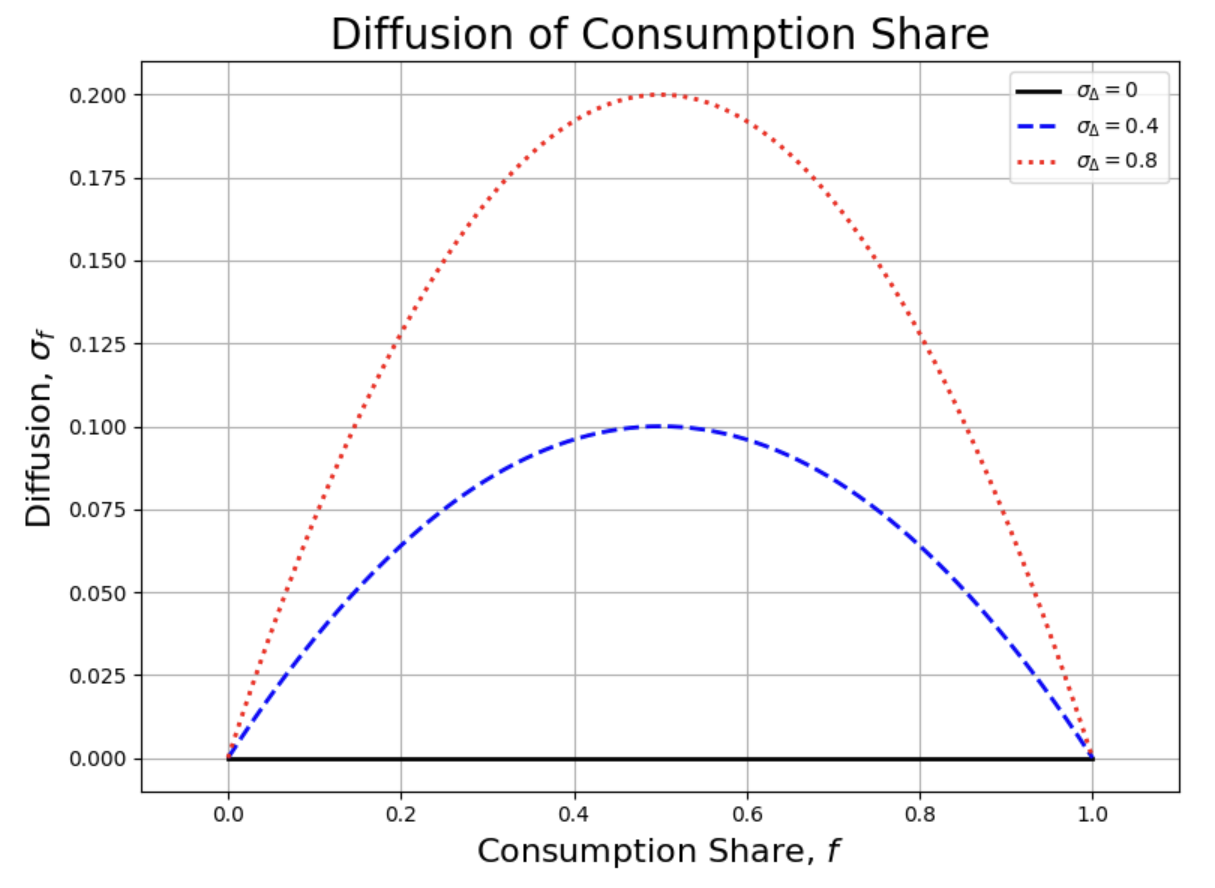
\includegraphics[width=.3\textwidth]{figuresJFE/ConsumptionShareDiffusion.png} &
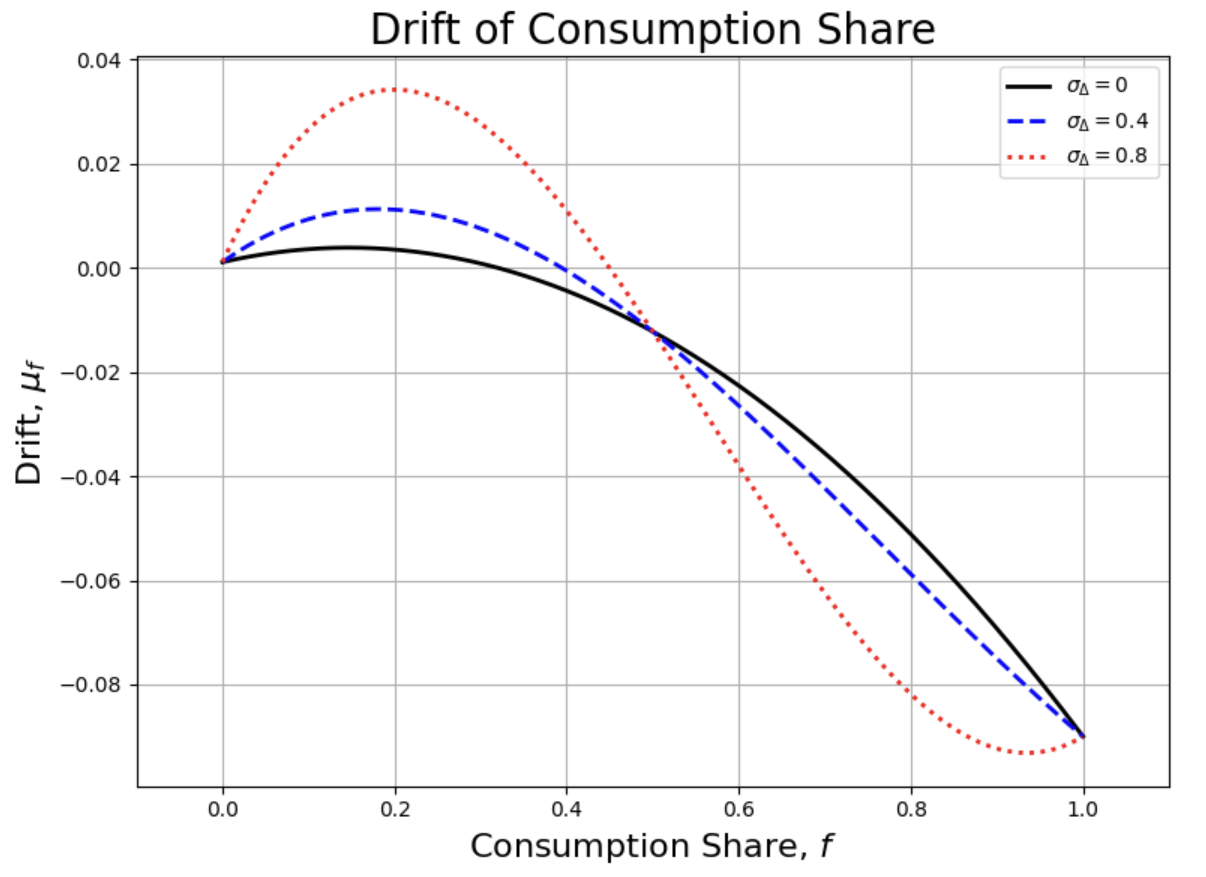
\includegraphics[width=.3\textwidth]{figuresJFE/ConsumptionShareDrift.png} \\
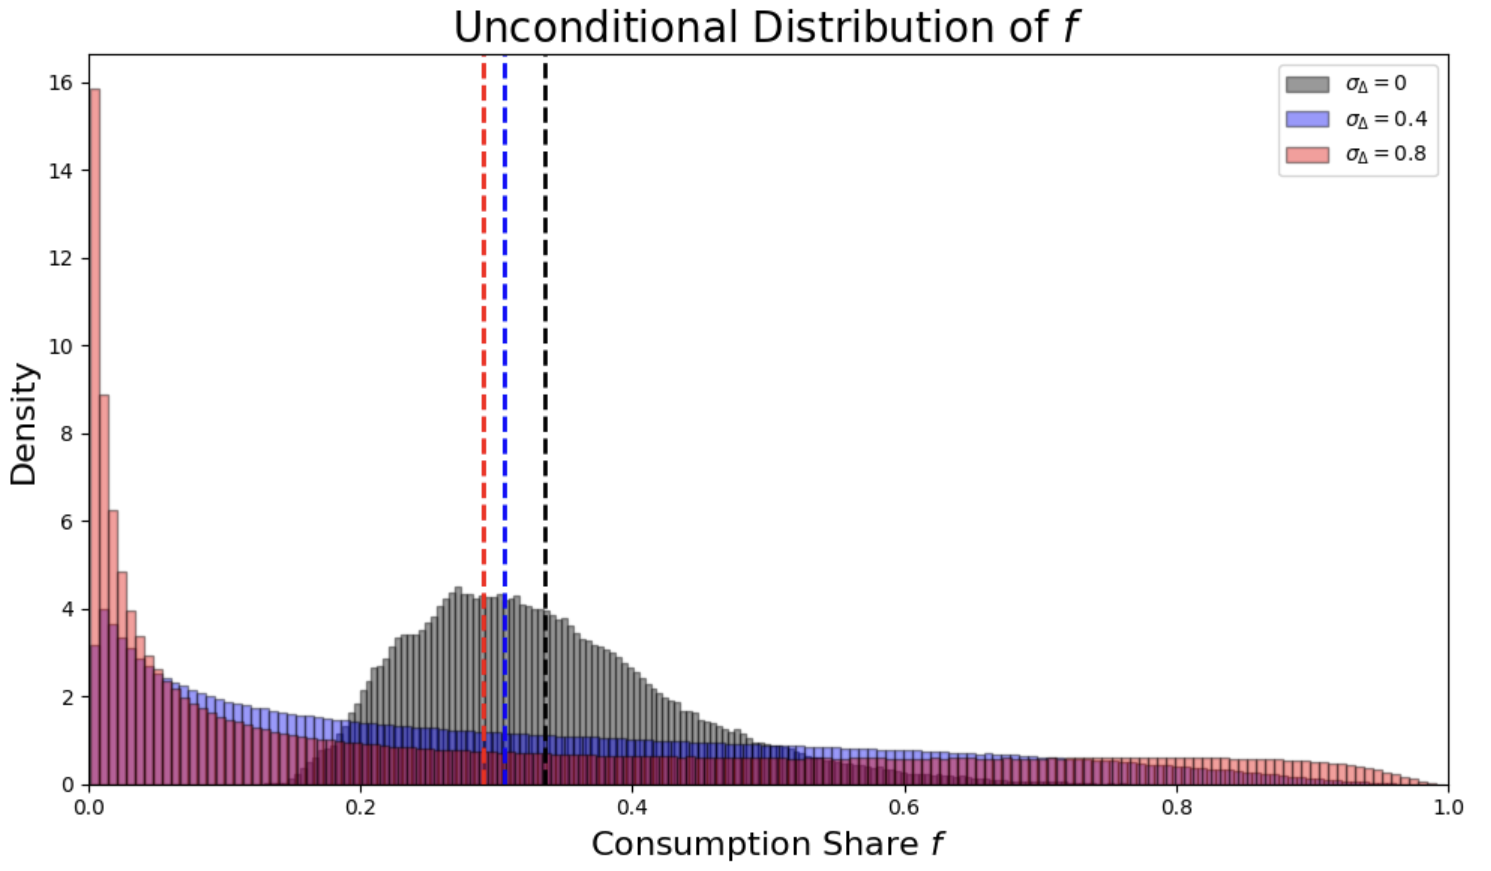
\includegraphics[width=.3\textwidth]{figuresJFE/HistConsumptionShare.png} &
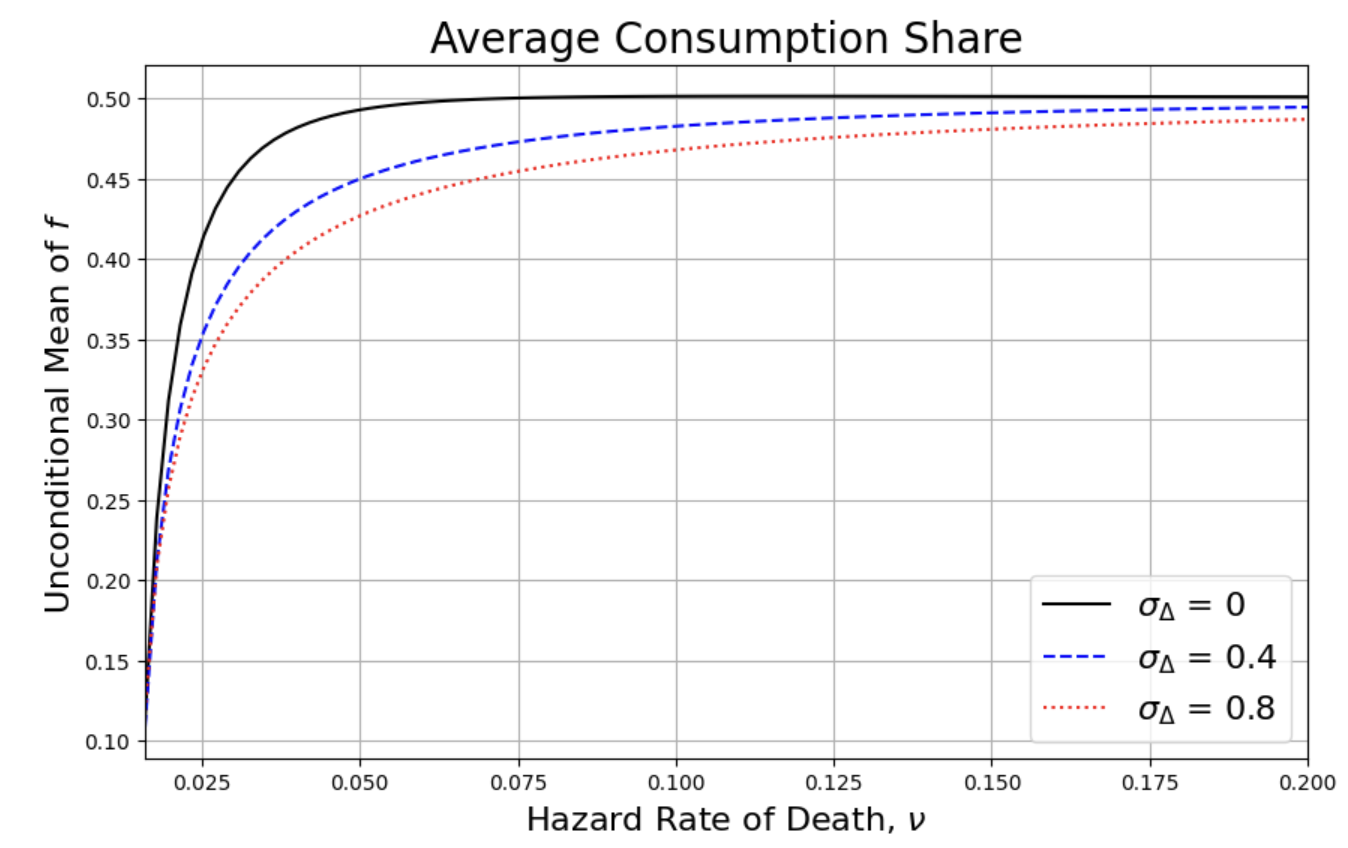
\includegraphics[width=.3\textwidth]{figuresJFE/AverageConsumptionShare.png}
\end{tabular}
\caption{\textbf{The consumption share.} \footnotesize{The top left graph shows the volatility $\sigma_{f,t}$ and the top right graph shows the drift $\mu_{f,t}$ of the consumption share dynamics as a function of the consumption share for three levels of disagreement $\sigma_{\Delta}$. The drift of the consumption share $\mu_{f,t}$ in the top right graph depends on the fraction of patient newborns $\alpha_t$ which is fixed at 0.5. The left graph shows the unconditional distribution of the consumption share of patient investors $\tilde{f}$ and the right graph shows the unconditional mean of the consumption share of patient investors $\mathrm{E}[\tilde{f}]$ as a function of the birth/mortality rate $\nu$. The histograms and unconditional means in the bottom row are based 500K years of monthly observations for each value of disagreement $\sigma_{\Delta}$.}} \label{fig:ConsumptionShare} 
\end{figure}

There are three economic effects that influence the consumption share drift, $\mu_{f,t}$, that is shown for different disagreement $\sigma_{\Delta}$ as a function of $f_t$ in the right graph of Figure \ref{fig:ConsumptionShare}. Specifically, there is (i) an OLG effect, (ii) a preference heterogeneity effect, (iii) and a disagreement effect. The first term of the drift in equation (\ref{eq:muf}), which is due to the OLG effect, leads to the time variation of the drift even without disagreement and it does not vanish when the consumption share approaches 0 or 1
because every instant new agents are born and the stochastic fraction, $\alpha_t$, measures how many of them are patient. Hence, the OLG effect leads to reflecting boundaries at 0 or 1 and to a stationary distribution of the consumption share, $f_t$. Moreover, the push upward at the lower bound is on average smaller than the push downward at the upper bound, that is,  $-0.09 dt$ vs $0.0011 dt$ in the top right graph of Figure \ref{fig:ConsumptionShare}. This holds more generally because the downward push when $f_t$ approaches one ($- \mathrm{E}[ \lim_{f_t \to 1} \mu_{f,t}] =   \nu \left( 1 - \mathrm{E}[\alpha_t ] \right)  (\rho^b+\nu) \phi^a$) is greater or equal to the upward push when $f_t$ approaches zero ($\mathrm{E}[ \lim_{f_t \to 0} \mu_{f,t}] =  \nu \mathrm{E}[\alpha_t ]  (\rho^a+\nu)  \phi^b$).
The average fraction of newborn patient investors is the same as for impatient investors, and so the economic reason for the different boundary behavior is twofold. First, impatient investors consume at a higher rate out of their initial wealth. Second, initial wealth is more valuable at the extinction boundary for impatient investors, where patient investors have all the price impact, and so valuation ratios are higher.  

The second term of the drift in Equation (\ref{eq:muf}) is due to investors having different time discount rates, and is always positive because $\rho^b>\rho^a$. This upward drift reflects the market selection force that favors the patient agent who saves more than the impatient agent, which in an infinite-horizon economy would lead to extinction of the impatient agent.  The third term of the drift in Equation (\ref{eq:muf}) is due to disagreement and disappears if the consumption share is 0 or 1 because neither patient nor impatient investors have someone to speculate with at the extinction boundaries.   In stark contrast to the consumption share volatility, disagreement has no effect on the drift when the consumption share is 0.5 because from the econometricians' perspective speculating on the demand shock is a fair gamble in this case and, hence, neither patient nor impatient investors' financial wealth, and, thus, consumption share is expected to change. 

We simulate $500,000$ years of monthly data for the consumption share $f_t$ using its dynamics given in Proposition \ref{prop:df} for three levels of disagreement $\sigma_{\Delta}$. Figure \ref{fig:ConsumptionShare} shows the histogram of $\tilde{f}$. In an infinite-horizon economy, this distribution would not exist, with the share converging to zero or one. The black dashed line indicates an unconditional mean of $\tilde{f}$ at $33.4\%$ without disagreement, below the $50\%$ mean of newborn patient investors $\mathrm{E}[ \alpha_t]$, as the OLG effect outweighs the market selection force.  
 

 

Disagreement further reduces the average consumption share of patient investors because speculation leads to large and persistent wealth swings, and thus higher probabilities of very low consumption shares. This effect results in long-run means of $\tilde{f}$ even further below $50\%$ as disagreement increases, shown in Figure \ref{fig:ConsumptionShare} (bottom left). The unconditional mean drops from $33.4\%$ without disagreement (black line), to $31.7\%$  with medium ($\sigma_{\Delta}= 0.4$, blue), and to $29.0\%$  with high disagreement ($\sigma_{\Delta}= 0.8$, red). Disagreement also increases the volatility of consumption shares from $10\%$ to $24.5\%$ and $29.4\%$, significantly increasing the likelihood of extreme consumption share realizations. The bottom right graph of Figure \ref{fig:ConsumptionShare} shows the unconditional mean of $\tilde{f}$ as a function of the birth/mortality rate $\nu$, ranging from $0.016$ to $0.2$. As $\nu$ increases, the patient type's consumption share approaches the mean of newborn patient investors, since shorter agent lifespans reduce the impact of market selection.\footnote{In an alternative calibration (Internet Appendix) with $\rho^a = 0.001$ and $\rho^B = 0.05$, we consider the infinitely lived case ($\nu = 0$), where disagreement leads to a non-monotonic relation: the most patient initially dominates, then the mean dips below $0.5$ before rising toward the unconditional mean of $\alpha$.}


\subsection{Valuation Ratio, Risk-free Rate, and Market Price of Demand Risk}

In equilibrium, the wealth-consumption ratio, the risk-free rate, and the market price of demand shocks are all affine functions of the consumption share \( \tilde{f} \). Therefore, these quantities inherit the properties of the unconditional distribution of \( \tilde{f} \), which we now briefly discuss.

From Corollary \ref{corollary:affine}, we know that the wealth-consumption ratio is strictly increasing in \( \tilde{f} \). Consequently, as disagreement increases, the unconditional mean of the wealth-consumption ratio \( \tilde{\phi} \) decreases, while its volatility increases. In other words, disagreement reduces the average valuation ratio and makes it more volatile. Moreover, the probability of observing a very low valuation ratio increases significantly with higher disagreement.

Similarly, Corollary \ref{corollary:affine} shows that the risk-free rate is strictly decreasing in \( \tilde{f} \). Thus, increasing disagreement raises the average interest rate and makes it more volatile. However, unlike the substantial increase in stock market volatility with greater disagreement, the effect on interest rate volatility is moderate. However, the likelihood of experiencing very low or high risk-free rates increases notably with greater disagreement.

The market price of demand risk \( \tilde{\theta}_{\alpha} \) is a strictly decreasing linear function of the consumption share \( \tilde{f} \). From Equation (\ref{theta_alphat}), its unconditional mean, $\mathrm{E}^{\sigma_{\Delta}} \left[ \tilde{\theta}_{\alpha} \right] = \sigma_{\Delta}\left( 0.5 - \mathrm{E}^{\sigma_{\Delta}} \left[ \tilde{f} \right] \right)$, is a nonlinear function of \( \sigma_{\Delta}\).
As \( \sigma_{\Delta}\) increases, the unconditional mean of the market price of demand risk initially decreases, then becomes positive, and is positive at the baseline setting \( \sigma_{\Delta}= 0.8 \).



 


\subsection{Bond and Stock Returns} \label{sec:StockBondDynamics}

In this subsection, we discuss the properties of bond and stock returns. We obtain closed-form solutions for the price of the stock market and consol bond and present their return dynamics in the next proposition. 
\begin{prop}[Consol and Stock Market]\label{prop:stockmarket}
The price of the consol is $B_t^C=\phi_t$ and its return dynamics are $ d R^C_t = \left( r_t + \lambda_{R^C,t} \right) \: dt + \sigma_{R^C,t}^{\alpha} \: dZ_{\alpha,t}$ with $\sigma_{R^C,t}^{\alpha}    = \frac{\phi^a - \phi^b}{\phi_t}  f_t \left(1-f_t\right)  \sigma_{\Delta} \geq 0$ and  $\lambda_{R^C,t} = \sigma_{R^C,t}^{\alpha} \theta_{\alpha,t}$.
The loading of the consol on the demand shock attains its maximum at $f_{\text{max}}=\left(1+\sqrt{\frac{\nu+ \rho^b}{\nu+ \rho^a}}\right)^{-1}\leq 0.5$. The stock market price is $\phi_t Y_t$ and the return dynamics are $d R^S_t = \left( r_t + \lambda_{R^S,t} \right) \: dt + \sigma^Y_{R^S,t} \: dZ_{Y,t}+  \sigma_{R^S,t}^{\alpha} \: dZ_{\alpha,t}$ with $\sigma^Y_{R^S,t} = \sigma_Y$, $\sigma_{R^S,t}^{\alpha} = \sigma_{R^S,t}^{\alpha}$, and $\lambda_{R^S,t} = \sigma_Y^2  + \lambda^{\alpha}_{R,t}$.
\end{prop}
We do not have closed-form solutions for the prices of discount bonds, and thus we use Monte Carlo simulations to determine the diffusion coefficient of the instantaneous discount bond return with maturity $T$ defined as $\sigma_{R^T,t}$. Hence, the risk premium of the discount bond is $\lambda_{R^T,t} = \theta_{\alpha,t}\sigma_{R^T,t}$. Figure \ref{fig:VolaRiskPremium2f} shows the volatility (left plot) and the risk premia (right plot) of bonds with maturities ranging from one to ten years, the consol bond, and the stock market as functions of the consumption share, $f_t$. %Instead of referring to loading of the consol on the demand shock as $\sigma_{R^{\alpha},t}^{\alpha}$ we will use the fact that it has the same loading as the stock market and therefore use $\sigma_{R,t}^{\alpha}$.
\begin{figure}[htbp]
\centering
\vspace{0.1in}
\begin{tabular}{cc}
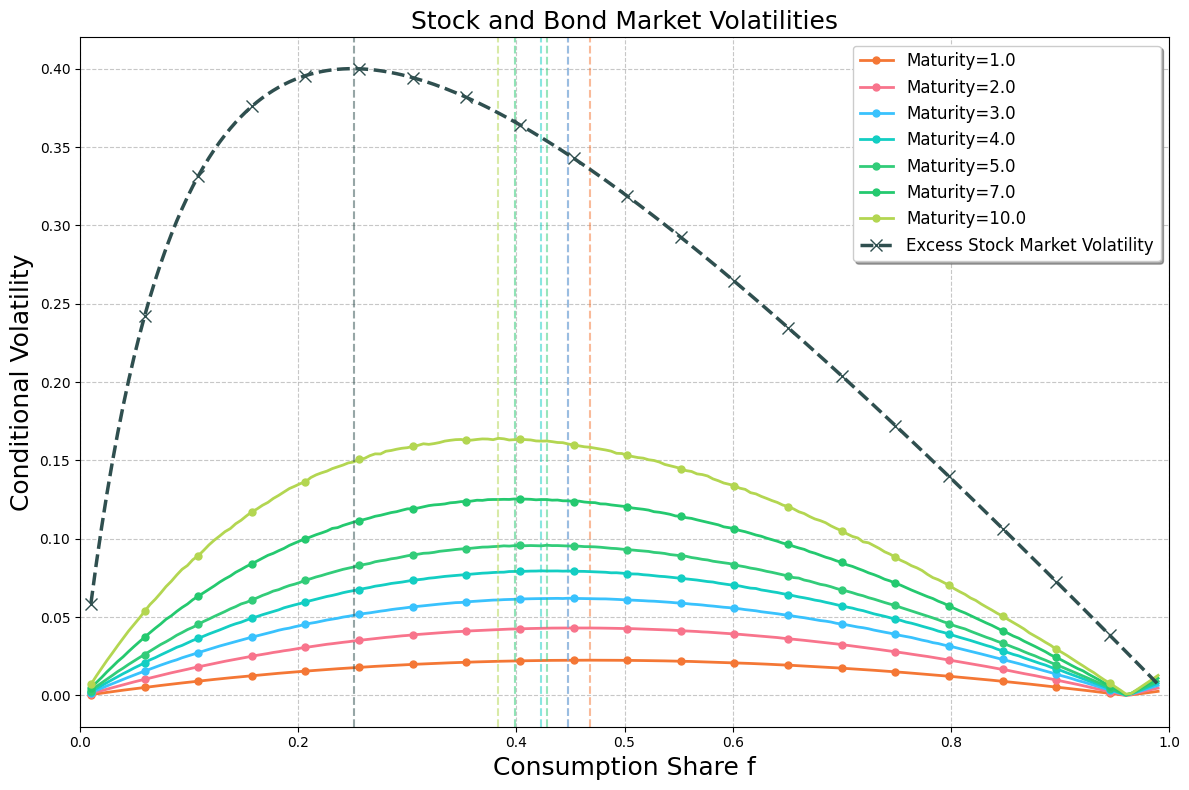
\includegraphics[width=.45\textwidth]{figures/volAPV3.png} &
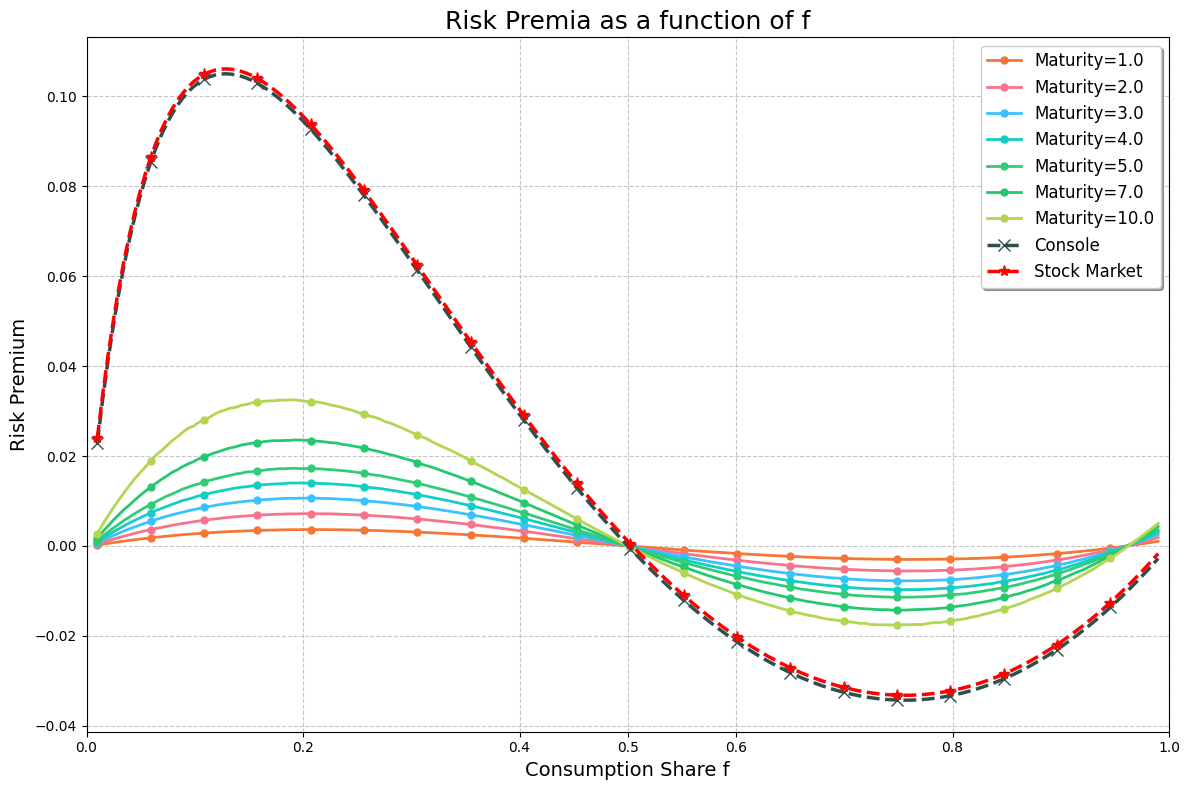
\includegraphics[width=.45\textwidth]{figures/RPV3.png}
\end{tabular}
\caption{\textbf{Conditional Return volatility and risk premium of bonds and stocks.} \footnotesize{The left graph shows bond return volatility and the right graphs shows the bond risk premium as a function of the consumption share $f_t$ for different maturities. In all figures we keep $\alpha = 0.5$.}} \label{fig:VolaRiskPremium2f}  
 \end{figure}

If there is no disagreement, then the instantaneous return of the consol is not exposed to the demand shock and, thus, locally risk-free. Disagreement and the resulting speculative trade increases the exposure to the demand shock, and so leads to volatile bond returns. Reducing the maturity of the bond lowers the exposure to demand shock risk, and thus lowers the volatility of the bond. The bond return exposure to demand shocks vanishes if the consumption share approaches either zero or one because in this case investors have no one to speculate with. Importantly, the volatility of the consol (and the stock market) is maximized at the value $f_{\text{max}} = 0.25$ (vertical black line) rather than at the peak of the speculative potential of investors when $f=0.5$. %Intuitively, the relative impact of bond and stock speculation is higher for lower valuation ratios which coincides with low consumption shares of patient investors. 
Shorter bond maturities shift this peak closer to $0.5$.\footnote{The short rate volatility, being linear in the consumption share, peaks when consumption volatility is at its maximum, which occurs at $f_t = 0.5$.}  Stock market volatility primarily reflects consol volatility, inheriting all its characteristics; as a result, the stock market exhibits excess volatility that mirrors the fluctuations observed in a consol bond.\footnote{Section \ref{sec:Extensions}.\ref{sec:GeneralDD} discusses extensions to our model that reduce this co-movement, leading to distinct differences between stock market and bond volatilities as well as risk premia.}




The right plot of Figure \ref{fig:VolaRiskPremium2f} shows risk premia conditional on the consumption share \( f \). When the consumption shares of patient and impatient investors are equal (\( f = 0.5 \)), the market price of demand shock risk vanishes. In this case, bond risk premia are zero because bonds are exposed only to demand shocks (and the equity premium is minimal due to the small market price of output risk under log utility). The conditional bond risk premium is positive when \( f_t < 0.5 \) and negative when \( f_t > 0.5 \). Importantly, bonds and stocks have a higher exposure to demand shock risk when \( f_t < 0.5 \), making the absolute value of the risk premium much higher in this scenario. Therefore, the stock market risk premium is not monotonic in the consumption share. Moreover, it is zero at the extinction boundaries \( f = 0 \) and \( f = 1 \), where exposure to demand shock risk disappears.

Although the conditional risk premia are positive for \( f_t < 0.5 \) and negative for \( f_t > 0.5 \), we can explain why the unconditional bond and stock risk premia are positive and increase with demand disagreement, as shown in Figure \ref{fig:UnconditionalAP}, along with an unconditional upward sloping yield curve. This arises from the unconditional risk premium equation:
\[
\mathrm{E} \left[ \tilde{\lambda} \right] = \mathrm{E} \left[ \tilde{\sigma}_{\alpha} \right] \mathrm{E} \left[ \tilde{\theta}_{\alpha} \right] + \mathrm{Cov} \left( \tilde{\sigma}_{\alpha}, \tilde{\theta}_{\alpha} \right),
\]
where \( \tilde{\lambda} \) is the risk premium and \( \tilde{\sigma}_{\alpha} \) is the demand risk exposure of a stock or bond. The positive unconditional risk premium results from two factors: (i) \(\mathrm{E} \left[ \tilde{\sigma}_{\alpha} \right] \mathrm{E} \left[ \tilde{\theta}_{\alpha} \right] > 0\) because the expected consumption share is below \( 0.5 \) and demand risk exposure is always positive; and (ii) \(\mathrm{Cov} \left( \tilde{\sigma}_{\alpha}, \tilde{\theta}_{\alpha} \right) > 0\) because maximum volatility occurs when \( f_t < 0.5 \), creating a positive correlation between risk exposure and the price of risk. Increased disagreement amplifies both effects, leading to higher unconditional asset risk premia.

The upward-sloping yield curve for maturities between one and ten years results from the peak in volatility shifting to lower consumption shares as bond maturity increases. This shift enhances the covariance with the price of demand shocks, increasing the risk premium for longer-maturity bonds.

 
 





\subsection{Yield Volatility and Bond Return Predictability}\label{sec:YieldVolaANDPredictability}

In this section we show empirically and in our model, that higher demand disagreement is robustly associated with greater yield volatility and predicts higher excess bond returns. 


We find a strong, positive relationship between demand disagreement and the volatility of discount bond yields across maturities from one to five years. In the data, we estimate nominal yield volatility using an AR(1)-GARCH(1,1) model and regress it on our measure of demand disagreement, as described in Section~\ref{sec:empirics}.\ref{sec:measuredemanddis}. In the model, where disagreement is entirely unrelated to macroeconomic fundamentals, demand disagreement reflects differences in one-year real short-rate forecasts between patient and impatient investors. Because there are no closed-form solutions, we use Monte Carlo simulations to compute both conditional yield volatility and demand disagreement. Table~\ref{table:regvola} shows that, both empirically and in the model, higher demand disagreement is consistently associated with higher yield volatility at all maturities. Quantitatively, a one-standard deviation increase in demand disagreement raises yield volatility by about 0.7 standard deviations in the data and nearly one-for-one in the model. The positive relationship in the data is robust to alternative disagreement measures and remains significant after controlling for yields and macroeconomic disagreement, as shown in Tables~8–11 of the Internet Appendix.

\begin{table}[h!]
\centering
\begin{tabular}{lccccc}
\toprule
\textbf{Maturity} & \textbf{1} & \textbf{2} & \textbf{3} & \textbf{4} & \textbf{5} \\ 
\midrule
Data   & 0.7334 & 0.7284 & 0.7204 & 0.6978  & 0.6618 \\ 
    & (14.108) & (13.902) & (13.584) & (12.738) & (11.544) \\ 
\midrule
Model  & 0.9938 & 0.9937 & 0.9928 & 0.9913 & 0.9892 \\ 
\bottomrule
& & & & & \\
\end{tabular}
\caption{\textbf{Yield Volatility Regression Coefficients.} This table presents the standardized regression coefficients of nominal yield volatility for discount bonds with maturities from one to five years, regressed on yield disagreement due to demand disagreement as implied by both the model and the data. In the model, yield volatility is estimated using a simulation of 500,000 years of data, regressing actual conditional volatility on yield disagreement based on one-year real yield forecasts. In the empirical analysis, nominal yield volatility is estimated using an AR(1)-GARCH(1,1) model and regressed on the demand disagreement measure constructed in Section~\ref{sec:empirics}.\ref{sec:measuredemanddis}. The model's standardized coefficients (population values) are consistent with those observed in the data. Newey-West corrected standard errors with four lags are used, and t-statistics for the data are reported in brackets.}
\label{table:regvola}
\end{table}

We also find a strong, positive relationship between demand disagreement and future excess bond returns across maturities from two to five years. In the data, we define the excess return of a $T$-year discount bond as the one-year holding period return of the $T$-year bond in excess of the one-year yield, and regress these on our measure of demand disagreement, as described in Section~\ref{sec:empirics}.\ref{sec:measuredemanddis}. In the model, we use Monte Carlo simulations to compute both the model-implied bond risk premium and demand disagreement. Table~\ref{table:regRP} shows that both empirically and in the model, a higher demand disagreement is consistently associated with higher future bond risk premia at all maturities. Quantitatively, the standardized coefficients in the data are substantial and statistically significant, while the model coefficients, though smaller, are consistent with the empirical findings. This predictive relationship in the data is robust to alternative disagreement measures and remains significant after controlling for yields and macroeconomic disagreement, as demonstrated in the Internet Appendix (see Tables 12-15 of the Internet Appendix). Notably, while disagreement spanned by macroeconomic fundamentals is associated with higher yield volatility, it does not predict bond excess returns, underscoring the unique predictive power of demand disagreement (see Table 10 for yield volatility and Table 14 for bond return predictability in the Internet Appendix).

 

\begin{table}[h!]
\centering
\begin{tabular}{lcccc}
\toprule
\textbf{Maturity} & \textbf{2} & \textbf{3} & \textbf{4} & \textbf{5} \\ 
\midrule
Data   & 0.4364  &  0.4085  & 0.3932  & 0.3837  \\ 
       & (5.845) &  (5.361) & (5.084) & (4.922) \\ 
\midrule
Model  & 0.1510  & 0.1505  & 0.1494  & 0.1478  \\ 
\bottomrule
       &   &    &   &   \\ 
\end{tabular}
\caption{\textbf{Bond Risk Premium Regression Coefficients.} This table presents the standardized regression coefficients of excess bond returns for discount bonds with maturities, $T$,  ranging from two to five years, regressed on yield disagreement due to demand disagreement as implied by both the model and the data. In the model, we use a simulation of $500,000$ years of data to regress the instantaneous bond risk premium, $\lambda_{R^T,t}$, on yield disagreement based on one-year real yield forecasts, as all yield disagreement in the model arises from demand disagreement. In the empirical analysis, bond risk premia are calculated as $rx^{(T)}_{t,t+4} = T y^{(T)}_{t} - (T-4)y^{(T-4)}_{t+4} - y^{(1)}_{t}$, where each period is a quarter, and are regressed on our demand disagreement measure constructed in Section~\ref{sec:empirics}.\ref{sec:measuredemanddis}. The standardized coefficients from both the model (population values) and the data are reported. Newey-West corrected standard errors with four lags are used, and t-statistics for the empirical data are reported in brackets. The model's coefficients are consistent with those observed in the data.}
\label{table:regRP}
\end{table}




\subsection{Estimating Latent States and Assessing Model Fit}\label{sec:backout}



We show in this section that, despite its parsimony, our demand disagreement model - with just one exogenous and one endogenous state variable, both driven by a single demand shock - delivers remarkable explanatory power for bond market dynamics, particularly for bond risk premia and the yield curve slope.


Our demand disagreement model features two latent state variables: the exogenous fraction of patient newborn investors ($\alpha_t$) and the endogenous consumption share of patient investors ($f_t$), both driven by a single Brownian shock ($Z_{\alpha,t}$). To estimate these unobservable states, we use the Unscented Kalman Filter (UKF) with only two observable time series: our demand disagreement measure and the two-year Treasury Inflation-Protected Security (TIPS) yield. We intentionally exclude longer-maturity TIPS yields (3, 5, 7, and 10 years) and nominal bond yields in the estimation for out-of-sample validation. This filtering approach is necessary due to the nonlinear relationship between the observables and the latent state variables.\footnote{For a detailed explanation of the estimation using the Unscented Kalman Filter, please refer to the Internet Appendix.}

\begin{figure}[htbp]
\centering
\begin{tabular}{cc}
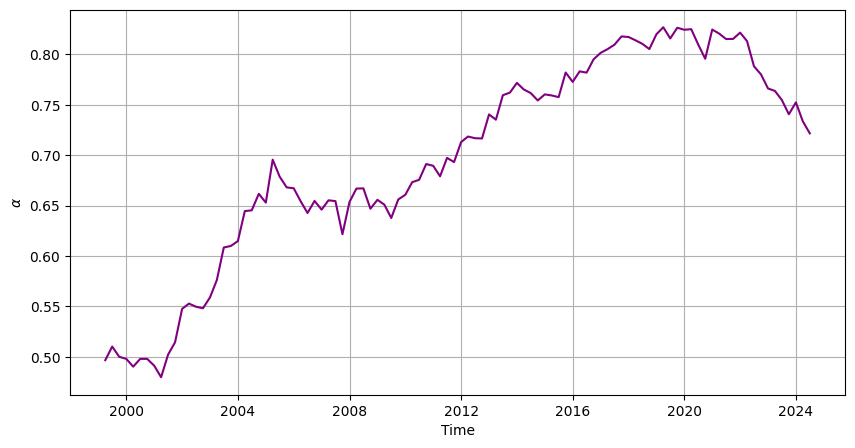
\includegraphics[width=.45\textwidth]{figures/alphaFilter.png} 
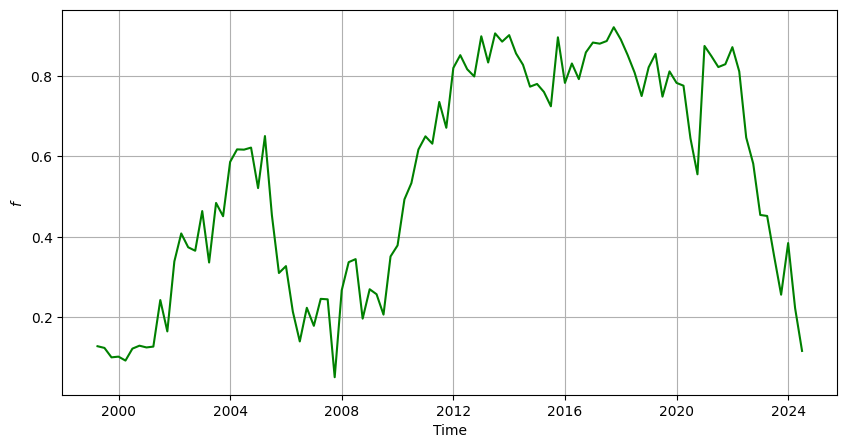
\includegraphics[width=.45\textwidth]{figures/ffilter.png} \\ 
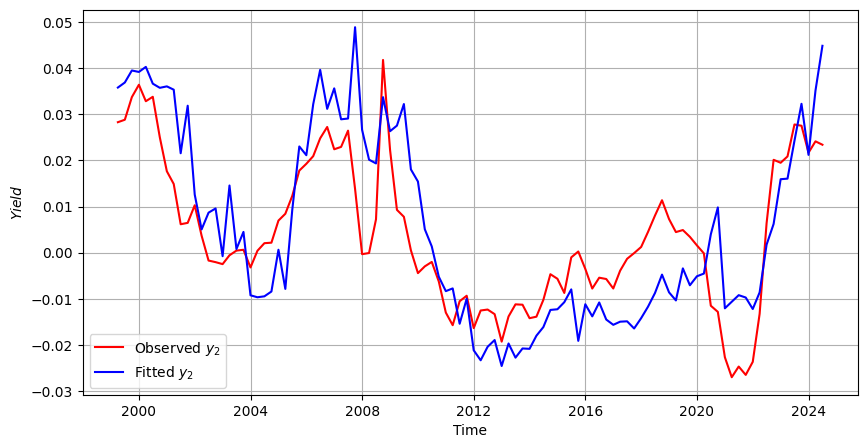
\includegraphics[width=.45\textwidth]{figures/yieldfilter.png} 
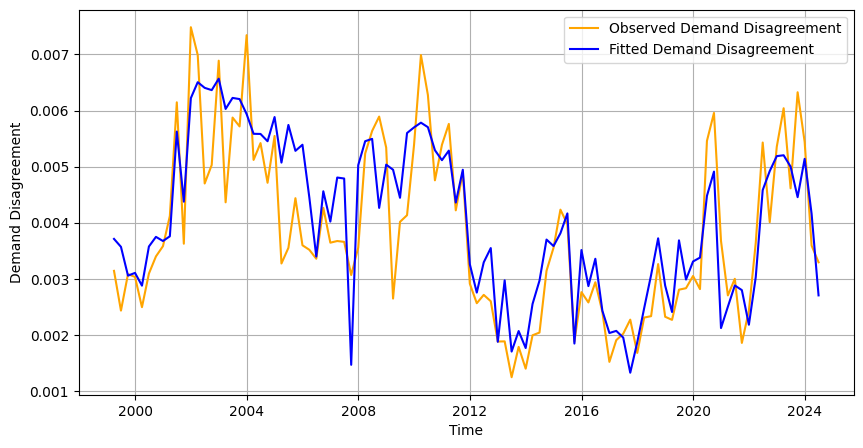
\includegraphics[width=.45\textwidth]{figures/DDfilter.png} \\ 
\end{tabular}
\caption{\textbf{Estimated state variables and fit to demand disagreement and the two year yield.} \footnotesize{The figure shows the estimated $\alpha$ (top-left), the estimated $f$ (top-right), the observed and implied two year real yield (bottom-left) and the observed and implied demand disagreement (bottom-left). We estimate the latent state variables using UKF. The observation equations are $y_t = h(l_t, f_t) + e_{y,t}$ and $DD_t = g(l_t,f_t) + e_{DD,t}$. We estimate the model using $l_t$ rather than $\alpha_t$.  We use the Euler discretization of the latent state variables with quarterly frequency as in the data. We assume a diagonal variance-covariance matrix for the observation noise with $Var(e_{y,t}) = 0.001 * var(y_{2,t})$ and $Var(e_{DD,t}) = 0.0005 * var(DD_t)$, We also assume a diagonal variance-covariance matrix of the prior variance in the two state variables with a variance of both set to $0.01$. We use data from 1999Q1-2024Q2 in the filtering.}}  \label{fig:UKFalphaandf}
\end{figure}
The plot on the top left of Figure \ref{fig:UKFalphaandf} shows an upward trend in implied $\alpha$ from 1999 to 2022, indicating an increasing fraction of better savers entering the economy. The consumption share exhibits similar but less pronounced trends. While the fraction of patient newborns has risen above the long-run mean, increasing the demand for savings, the consumption share is less persistent and more volatile than the newborn fraction. Notable fluctuations include a significant drop in the share of patient agents' consumption around 2005, coinciding with a temporary $\alpha$ decline and a sharp $f_t$ decrease in recent years as real rates increased. The bottom panels demonstrate that, despite the parsimony of the model having only one shock to the exogenous and endogenous state variables, the filtered model provides a reasonable fit to both the observed demand disagreement and the real two-year yield. Notably, because both state variables are driven by a single shock in this nonlinear model, it is less flexible in fitting both observables.

Building on these filtered state variables, we generate model-implied time series for real yields (2, 3, 5, 7, and 10 years), their estimated AR(1)-GARCH(1,1) volatilities, and realized annual holding period returns of nominal bonds in excess of the one-year nominal yield. To evaluate the empirical performance of the model, we regress the observed data for these variables on their model-implied counterparts. Table~\ref{table:UKFOOS} summarizes these results. In an ideal scenario, the regression slope would be one and $R^2$ high, indicating a great fit.\footnote{We do not expect a very high $R^2$ for risk premia since we regress realized returns in the data on the model implied risk premium.} While omitted factors and the simplicity of the model naturally limit explanatory power, the results are surprisingly strong: all regression coefficients are positive and statistically significant, and for both nominal bond risk premia and the slope of the real yield curve, we cannot reject the null hypothesis that the coefficient equals one. The model also captures the cyclicality of the slope of the real yield curve, a challenging feature for general equilibrium models, and effectively predicts bond risk premia over 98 quarters. Although real yield volatilities show weaker explanatory power, especially at the two-year maturity, the overall findings underscore the model's ability to capture key features of the data with minimal structure and only a single source of uncertainty.



\begin{table}[ht]
    \centering
    \begin{tabular}{lccccccccc}
        \toprule
        \multirow{2}{*}{\textbf{Maturity}} & \multicolumn{3}{c}{\textbf{Real Yields}} & \multicolumn{3}{c}{\textbf{Real Yield Volatilities}} & \multicolumn{3}{c}{\textbf{Nominal Bond Risk Premia}} \\
        \cmidrule(lr){2-4} \cmidrule(lr){5-7} \cmidrule(lr){8-10}
        & \textbf{Coeff.} & \textbf{Std. Dev.} & \textbf{R$^2$} & \textbf{Coeff.} & \textbf{Std. Dev.} & \textbf{R$^2$} & \textbf{Coeff.} & \textbf{Std. Dev.} & \textbf{R$^2$} \\
        \midrule
        2 years  & 0.621 & 0.062 & 0.667 & 0.141 & 0.093 & 0.035 & 1.354 & 0.543 & 0.178 \\
        3 years  & 0.593 & 0.057 & 0.694 & 0.156 & 0.073 & 0.086 & 1.540 & 0.672 & 0.143 \\
        5 years  & 0.558 & 0.054 & 0.687 & 0.136 & 0.045 & 0.155 & 1.281 & 0.708 & 0.084 \\
        7 years  & 0.535 & 0.053 & 0.663 & 0.111 & 0.038 & 0.136 & --    & --    & --    \\
        10 years & 0.517 & 0.052 & 0.629 & 0.079 & 0.032 & 0.088 & --    & --    & --    \\
        Slope    & 1.147 & 0.275 & 0.236 & --    & --    & --    & --    & --    & --    \\ 
        \bottomrule
    \end{tabular}
    \vspace{0.5em}
    \caption{Regression Results: Yields, Yield Volatilities, and Bond Risk Premia}
    \label{table:UKFOOS}
    \begin{minipage}{0.95\textwidth}
        \footnotesize{The table displays regression results of observed data against model-implied values based on filtered $\alpha_t$ and $f_t$. Coefficients are estimated from the regression $y^{\text{Data}}_t = a + b y^{\text{Model}}_t + u_t$. Dashes indicate missing data for certain maturities. Although coefficients differ from one, their statistical significance and correct signs demonstrate that the model captures essential data features.}
    \end{minipage}
\end{table}

Finally, we note that the above filtering relies on our measure of demand disagreement (see Section \ref{sec:empirics} for details). In the Online Appendix, we present an alternative filtering approach that uses yield disagreement directly as an observable in the estimation. Because yield disagreement also reflects macroeconomic disagreement, we include an additional observation equation and latent state variable. Since our model does not feature macroeconomic disagreement, we assume it does not affect bond yields. The results from this alternative approach are very similar to those reported here.














 
\section{Discussion and Extensions}\label{sec:Extensions}

In this section, we explore potential extensions to our model that offer additional insight into asset pricing, as well as address some limitations of our current framework and potential improvements. Our primary goal has been to develop a tractable model with clear economic forces that reduces the strong correlation between fundamentals and asset returns, as well as the correlation between fundamental disagreement and returns that many models imply. Furthermore, we demonstrate that demand disagreement plays a significant role in bond pricing, both in the model and in the empirical data. A natural starting point to achieve these objectives is an exchange economy with log utility, and different time preferences.  Moreover, investors have dogmatic beliefs and a false consensus bias. While these simplifying assumptions improve model transparency and tractability, they involve certain trade-offs.

Here, we briefly discuss three possible extensions: (1) a more generalized form of demand disagreement, (2) time-varying disagreement, and (3) a production economy extension of our model. Through these extensions, we demonstrate that while our baseline model is intentionally simplistic, its core insights remain robust even within more generalized frameworks. For brevity, we present only an overview here, with detailed derivations and extended discussions available in the Internet Appendix.


 
\subsection{Demand Disagreement from Heterogeneous Risk Aversion} \label{sec:GeneralDD}

In this paper, we focus on demand disagreement that arises from differing beliefs about the future distribution of patient and impatient investors. This limits our model's ability to capture certain asset price moments, such as the equity premium. %Specifically, stock returns are exposed to (i) cash flow risk and (ii) the price risk of a consol---a perpetual bond with a time-dependent coupon rate:
In this framework, demand shocks only affect the yield curve, which implies that both the stock risk premium and its volatility are largely determined by the risk premium and volatility of the consol. This aligns with recent evidence from \cite{JVB:2021}, showing that duration-matched bond portfolios are as volatile as stocks and yield similar excess returns. Consequently, our analysis emphasizes the effects of demand disagreement on bond pricing.

There are several ways to extend our model to drive a wedge between stock and bond returns. First, allowing for preferences with constant relative risk aversion (CRRA) preferences and letting the two investor types differ in risk aversion would break this link. In this scenario, demand disagreement would also affect the pricing of fundamental (cash flow) shocks, as the effective risk aversion in the economy would become the consumption-weighted harmonic average of the risk aversions of the two types. Specifically, the market prices of output and demand risk would take the form \(\theta_{Y,t} = \mathcal{R}_t \sigma_Y\) and \(\theta_{\alpha,t} = -\bar{\sigma}^{\mathcal{R}}_{\Delta,t}\), with consumption- and risk-tolerance-weighted risk aversion and estimation error defined as:\footnote{See \cite{HeyerdahlLarsenIlledistch23} for derivations of a general OLG model with differences in beliefs and preferences.}
\begin{equation}
\mathcal{R}_t = \frac{1}{f_t \frac{1}{\gamma^a} + \left(1 - f_t\right) \frac{1}{\gamma^b}} \qquad \text{and} \qquad \bar{\sigma}^{\mathcal{R}}_{\Delta,t} = \frac{f_t \frac{1}{\gamma^a} \sigma_{\Delta}^a + \left(1 - f_t\right) \frac{1}{\gamma^b} \sigma_{\Delta}^b}{f_t \frac{1}{\gamma^a} + \left(1 - f_t\right) \frac{1}{\gamma^b}}.
\end{equation}
The consumption share, \(f_t\), would now depend on both fundamental output shocks from differences in risk aversion and demand shocks from distribution shifts of preference types. Additionally, the price of risk for output shocks, \(\theta_{Y,t}\), would indirectly reflect demand shocks through its dependence on consumption shares, leading to disagreement about the future risk premium for output shocks. This divergence would introduce a wedge between the stock and bond markets.

Another possible extension is to incorporate recursive preferences or to introduce output disagreement alongside demand disagreement. With recursive preferences, demand shocks would typically be priced even without demand disagreement. Moreover, allowing heterogeneity in time preferences, risk aversion, and the intertemporal elasticity of substitution (IES) would further increase the disconnect between stock and bond markets.



\subsection{Time-Varying Disagreement---Learning from Experience}\label{sec:TimeVaryingBeliefs}

Until now, we have assumed that agents have dogmatic beliefs about the long-run mean of \( l_t \), and thus the fraction of patient newborns, \( \alpha_t \). This leads to constant estimation errors and non-stochastic disagreement, a parsimonious approach given the exogenous nature of the process. Alternatively, one could assume exogenously that agents have differing beliefs about persistence, resulting in stochastic disagreement. Hence, we treat the estimation error for type \( i = a, b \) agents, \( \sigma_{\Delta,t}^i \), as stochastic, so that \( \sigma_{\Delta,t} = \sigma_{\Delta,t}^a - \sigma_{\Delta,t}^b \) captures the stochastic disagreement between types. Where closed-form solutions apply, substituting the constant \( \sigma_{\Delta}\) with \( \sigma_{\Delta,t} \) provides comparable results.

In the Internet Appendix, we endogenize disagreement through learning. Here, agents observe lifetime data to infer the long-run mean of \( l_t \), leading to time-varying, cohort-dependent disagreement. Using Bayes' rule and experience-based learning as in \cite{EGH18}, agents initially share identical priors for the unknown long run mean of $l_t$ but there is disagreement over time across birth cohorts. This results in a stochastic \( \sigma_{\Delta,t} \) without the assumption of a false consensus bias. Furthermore, consumption shares become cohort-dependent: older agents typically have higher consumption shares due to lower estimation errors. This approach reproduces the qualitative findings of the baseline model, extending it to accommodate richer dynamics in beliefs and consumption patterns across cohorts.

 

\subsection{Production Economies}\label{sec:Production}

Our prior analysis assumed an exchange economy with zero correlation between aggregate consumption and demand shocks, which naturally lacks a correlation puzzle. In the Internet Appendix, we extend this model to include production, following \cite{BrunnermeierSannikov2014} for capital dynamics and investment adjustment costs. Capital evolves as \( dK_t = \left(\psi(\iota_t) + \mu_K - \sigma_{\Delta}\right) K_t \, dt + \sigma_K K_t \, dZ_{K,t} \), where \( \psi(\iota) = \frac{\log(\kappa \iota + 1)}{\kappa} \) defines how the investment rate \( \iota_t \) influences capital growth. With \( \kappa \to 0 \), the adjustment costs disappear and the output, as a fraction of capital, is given by \( Y_t = a K_t \).

The production model shows that, with endogenous capital choice, the correlation puzzle remains. For a range of \( \kappa \) values, dividend-stock return correlations are low or negative, yet demand shock risk premia stay positive. Contrary to expectations, shocks negatively correlated with consumption growth do not inherently imply negative risk premia. The demand disagreement model highlights that speculative dynamics can reverse the price of risk, potentially intensifying the correlation puzzle in a production setting.





\section{Conclusion}\label{sec:conclusion}

We develop an overlapping generations (OLG) model in which the cross-sectional distribution of investor preferences and beliefs evolves over time. In our model, investors hold incomplete information and disagree on these changes, creating persistent disagreement about future asset demand—even when economic fundamentals are known. This demand disagreement gives rise to speculative trade that is disconnected from fundamentals, introducing priced demand shocks into the asset markets.  Demand disagreement accounts for the low correlation between asset returns and economic fundamentals and explains yield disagreements that are not driven by macroeconomic factors. Moreover, it increases risk premia in both stock and bond markets, generates an upward-sloping real yield curve, establishes a positive relationship between demand disagreement and yield volatilities, and produces bond risk premia that are predictable by yield disagreement. 


 \begingroup
    	\setstretch{1.21}
	\bibliographystyle{jf}
	\bibliography{OLGBeliefsAccepted}\label{references}
\endgroup   

\renewcommand{\baselinestretch}{1}  % linespacing, 2 doublespace
    
% Define aexample counter for JF style
\newcounter{aexample}

\appendix

 
\section{Appendix}\label{sec:Appendix}
\textbf{Proofs}
\begin{proof}[Proof of Proposition \ref{SDF}]
To solve for the  equilibrium stochastic discount factor, we insert optimal consumption from Equation (\ref{optimalconsumption}) into the aggregate resource constraint, $\int_{-\infty}^{t} \nu e^{-\nu (t-s )} (\alpha_s c^a_{s,t}+(1-\alpha_s) c^b_{s,t}) ds =  Y_t$ and rearrange terms. We get $\xi_t = \frac{X_t}{Y_t}$ where $X_t$ solves the integral equation 
\begin{equation}\label{eq:Xtapp}
	X_t =\int_{-\infty}^{t} \nu e^{-\nu \left(t-s\right)} \left(\alpha_s \beta^a_s e^{-\rho^a \left(t-s\right)}\frac{\eta^a_t}{\eta^a_s} +\left(1-\alpha_s\right)\beta^b_s e^{-\rho^b \left(t-s\right)} \frac{\eta^b_t}{\eta^b_s}\right)X_s ds.
\end{equation}
\end{proof}
\begin{proof}[Proof of Proposition \ref{prop:f}]
We use type $a$'s optimal consumption demand, $c^a_{s,t} = c_{s,s}e^{-\rho^a t} \frac{\eta^a_t}{\eta^a_s} \frac{\xi_s}{\xi_t}$ to get
\begin{equation}
    \xi_t X^a_t =  \int_{-\infty}^{t} \nu e^{-\left(\rho^a + \nu\right)\left(t-s\right)}\alpha_s \beta^a_s \frac{\eta^a_t}{\eta^a_s}X_s ds = \xi_t\int_{-\infty}^{t} \nu e^{-\left(\rho^a + \nu\right)\left(t-s\right)}\alpha_s c^a_{s,t} ds.
\end{equation}
Similarly, $X^b_t$ follows from optimal consumption of type $b$ agents. Hence, we get
\begin{equation}
    f_t = \frac{ \xi_t X^a_t }{  \xi_t X^a_t +  \xi_t X^b_t } =   \frac{X^a_t }{ X_t } 
\end{equation}
\end{proof}

\begin{proof}[Proof of Proposition \ref{prop_rtandtheta}]
Applying Ito's lemma to $X_t$ given in Equation (\ref{eq:Xtapp}) leads to 
\begin{equation}
    dX_t = \left(-\left(f_t\rho^a + \left(1-f_t\right)\rho^b\right) - \nu\left(1-\alpha_t \beta^a_t - \left(1-\alpha_t\right)\beta^b_t\right)\right)X_t dt + \mathcal{E}_{f}\left [ \sigma_{\Delta}  \right] X_t dZ_{\alpha,t},
\end{equation}
with $\mathcal{E}_{f} \left [ \sigma_{\Delta} \right] = f_t \sigma_{\Delta}^a  + \left(1-f_t\right)\sigma_{\Delta}^b$.  Applying Ito's lemma Ito's o $\xi_t = \frac{X_t}{Y_t}$ leads to
\begin{eqnarray}
    d\xi_t &=& \frac{dX_t}{Y_t} + X_td\left(\frac{1}{Y_t}\right) + \frac{dX_t}{Y_t}d\left(\frac{1}{Y_t}\right) \nonumber \\
    &=& \frac{X_t}{Y_t}\left(-\left(f_t\rho^a + \left(1-f_t\right)\rho^b\right) - \nu\left(1-\alpha_t \beta^a_t - \left(1-\alpha_t\right)\beta^b_t\right)\right)dt \nonumber \\
    && -\frac{X_t}{Y_t}\left( \mu_Y - \sigma_Y^2\right)dt - \frac{X_t}{Y_t}\left(\sigma_Y dZ_{Y,t} - \bar{\sigma}_{\Delta,t} X_t dZ_{\alpha,t}\right) \nonumber \\
    &=& \xi_t \left(-r_t dt - \theta_{Y,t}dZ_{Y,t}  - \theta_{\alpha,t}dZ_{\alpha,t}\right),
\end{eqnarray}
where $r_t$, $\theta_{\alpha,t}$ and $\theta_{Y,t}$ are as in Proposition \ref{prop_rtandtheta}.
\end{proof}



 

\begin{proof}[Proof of Proposition \ref{prop_PD}]
We have $c^i_t = \left(\rho^i + \nu\right) W^i_t$ for $i \in \left\{a,b\right\}$ and define $\phi^i = \frac{W^i_{s,t}}{c^i_{s,t}} = \frac{1}{\rho^i + \nu}$. To derive the wealth-consumption ratio, we multiply the consumption share $f_{t}$ and $(1-f_t)$ with $\phi^{a}$ and $\phi^{b}$, respectively. Then we add up both terms and impose market clearing to get
\begin{equation}
    \phi^{a} f_t + \phi^{b}\left(1-f_t\right) = \frac{W^a_t}{c^a_t}f_t + \frac{W^b_t}{c^b_t}\left(1-f_t\right) = \frac{W^a_t + W^b_t}{Y_t} = \frac{W_t}{Y_t}.
\end{equation}
Aggregate consumption and wealth of all agents of type $i$ are $c^i_t$ and $W^i_t$ for $i \in \left\{a,b\right\}$, respectively.
\end{proof}
\begin{proof}[Proof of Corollary \ref{corollary:affine}]
Taking the first derivative of (i) the risk-free rate $r(f)$ given in Equation \ref{rt}, the market price of demand shock risk $\theta_{\alpha}(f)$ given in Equation (\ref{theta_alphat}), and (iii) the wealth-consumption ratio $\phi(f)$ given in Proposition (\ref{prop_PD}) w.r.t. the consumption share $f$ proves the result. 
\end{proof}
\begin{proof}[Proof of Corollary \ref{corollary:consol}]
First, note that we can write, $\phi_t$, as 
\begin{equation}
    \begin{split}
    \phi_t &=  E_t\left[\int_{t}^{\infty} \frac{\xi_{u}}{\xi_t}e^{-\nu\left(u-t\right)}\frac{Y_u}{Y_t}du\right]  
     =  \int_{t}^{\infty} E_t\left[\frac{\xi_{u}}{\xi_t}e^{-\nu\left(u-t\right)}\frac{Y_u}{Y_t}\right]du \\
    &=  \int_{t}^{\infty} E_t\left[\frac{\hat{\xi}_{u}}{\hat{\xi}_t}\right]e^{-\nu\left(u-t\right)}E_t\left[e^{-\frac{1}{2}\sigma_Y^2\left(u-t\right) - \sigma_Y \left(Z_{Y,u} - Z_{Y,t}\right)}\frac{Y_u}{Y_t}\right]du    
     =  \int_{t}^{\infty}  e^{(\mu_Y - \sigma_Y^2 - \nu) (u-t)} B^u_{t}du
\end{split}
\end{equation}
where we have defined $\xi_t = \hat{\xi}_{t} e^{-\frac{1}{2}\sigma_Y^2 t - \sigma_Y \left(Z_{Y,u} - Z_{Y,t}\right)}$.
\end{proof}
 \begin{proof}[Proof of Proposition \ref{prop:df}]
 Applying Ito's lemma to the consumption share $f_t = \frac{X^a_t}{X_t}$ leads to its dynamics.
 \end{proof}
\begin{proof}[Proof of Proposition \ref{prop:stockmarket}]
 The wealth-consumption ratio is $\phi_t = \phi^{a} f_t + \phi^{b} (1-f_t)$ and thus applying It\^o's lemma to the price of the market portfolio $S_t = Y_t \phi_t$ and using the dynamics of the consumption share $f_t$ given in Proposition \ref{prop:df} leads to the exposures of stock market returns to the supply ($\sigma_{R,t}^Y$) and demand ($\sigma_{R,t}^{\alpha}$) shock as well as the risk premium $\lambda_{R,t}$. $\sigma_{R,t}^{\alpha}$ is a concave function of the consumption share $f_t$ and, thus, taking the first derivative w.r.t. f leads to the global maximum of the demand shock exposure and thus the the conditional stock market volatility.   
\end{proof}

 
 \end{document} 

